%!TEX root = ../thesis.tex
%*******************************************************************************
%****************************** Second Chapter *********************************
%*******************************************************************************

\chapter{Desarrollo de modelos predictorios para mutaciones puntuales}

\ifpdf
    \graphicspath{{Chapter2/Figs/Raster/}{Chapter2/Figs/PDF/}{Chapter2/Figs/}}
\else
    \graphicspath{{Chapter2/Figs/Vector/}{Chapter2/Figs/}}
\fi

El estudio del efecto de mutaciones puntuales en complejos de proteínas, es una de las problemáticas más estudiadas en los últimos años, enfocándose principalmente, en la evaluación de cambios en la estabilidad de la proteína mediante la variación de energía libre que la mutación provoca \cite{Schymkowitz2005,Pandurangan2017,rohl2004protein,Parthiban2006}. 

Diferentes modelos de clasificación han sido desarrollados para poder predecir cambios de energía libre, en base a algoritmos de aprendizaje supervisado o mediante técnicas de minería de datos, y así, determinar el efecto de la mutación en set de proteínas de interés \cite{Quan2016,Capriotti2008,Broom2017,Khan2010,vaisman,Getov2016,Capriotti2005}. No obstante, en casos más específicos, se han desarrollado modelos para proteínas exclusivas con el fin de asociar la mutación a un rasgo clínico \cite{article}. 

En ambos casos, es necesario construir set de datos con respuesta conocida para poder entrenar los modelos y así evaluar su desempeño. Los enfoques principales al desarrollo de descriptores se basan en propiedades fisicoquímicas y termodinámicas, así como también, el ambiente bajo el cual se encuentra la mutación \cite{Capriotti2005}. Sin embargo, dejan de lado, los componentes asociados a conceptos filogenéticos y la propensión a cambios de dicha mutación \cite{Olivera-Nappa2011}.

Dado a los modelos existentes y en vista a la necesidad de generar nuevos sistemas de clasificación para mutaciones puntuales en proteínas, debido al aumento considerable de reportes en los últimos años, se propone una nueva metodología para el diseño e implementación de evaluación de mutaciones en proteínas, describiéndolas desde los puntos de vista termodinámico y filogenético y usando algoritmos de aprendizaje supervisado como generadores de modelos, metodología la cual ha sido evaluada para generar clasificadores de propensión clínica de mutaciones en von Hippel Lindau.

A continuación, se describen algunas herramientas computacionales y su significancia para este estudio a la hora de comparar y analizar los resultados obtenidos, seguido además de los conceptos relacionados al aprendizaje supervisado, junto con la metodología desarrollada, los resultados y discusiones del proceso, así como también el uso de esto en casos particulares.


\section{Herramientas computacionales asociadas a evaluación de mutaciones}

Las herramientas computacionales asociadas a la evaluación de mutaciones puntuales se centran principalmente en el análisis de cómo ésta afecta a la estabilidad o la predicción de energía libre asociada a los residuos involucrados en la mutación.

\section{Aprendizaje de Máquinas}

Aprendizaje de Máquina, es una rama de la inteligencia artificial que tiene por objetivo el desarrollo de técnicas que permitan a los computadores aprender, es decir, generalizar comportamientos a partir de una información no estructurada suministrada en forma de ejemplos \cite{michie1994machine}. Aplicándose en diferentes campos de investigación: motores de búsqueda \cite{cooley1997web}, diagnósticos médicos \cite{7912315,ABDELAZIZ2018117}, detección de fraude en el uso de tarjetas de crédito, bioinformática \cite{juanito}, reconocimiento de patrones en imágenes \cite{imageA} y textos \cite{netzer2011reading,alm2005emotions}, etc. 


Los algoritmos de aprendizaje pueden clasificarse en dos grandes grupos \cite{michie1994machine}:

\begin{itemize}
	
	\item \textbf{Supervisados}: se cumple un rol de predicción, clasificación, asignación, etc. a un conjunto de elementos con características similares, por lo que los datos de entrada son conocidos.
	
	\item \textbf{No Supervisados}: su objetivo es agrupar en conjuntos con características similares los elementos de entrada dado los valores de estos atributos, en base a la asociación de patrones característicos que representen sus comportamientos.
\end{itemize}

A continuación se describen en forma general, los algoritmos de aprendizaje supervisados utilizados para el desarrollo de la metodología, explicando los conceptos bajo los que se basan y cómo estos entrenan y se emplean para predecir o clasificar nuevos ejemplos.

\subsection{Algoritmos de aprendizaje supervisado}

Existen diferentes algoritmos de aprendizaje supervisado, los cuales pueden ser asociados a la clasificación de un elemento o la predicción de valores, dependiendo el tipo de respuesta existente en el conjunto de datos a estudiar. En el caso de respuestas con distribución continua, se trabajan con algoritmos de regresión, mientras que si la respuesta es binaria o multiclase y es representada por variables categóricas, los algoritmos se basan en clasificadores \cite{michie1994machine}.

A su vez, también se pueden dividir con respecto a la forma en que se trata el problema, existiendo algoritmos basados en cálculos de distancia entre ejemplos (K-Vecinos Cercanos), otros que consideran transformaciones vectoriales y aplicaciones de funciones de kernel (Máquina Soporte de Vectores), así como también el uso de las características como entorno espacial de decisión (Árboles y métodos de ensamble) y aquellos que utilizan redes neuronales y trabajan en torno a cajas negras.

Cada uno de estos algoritmos es descrito a continuación, enfocándose tanto en el componente matemático asociado, así como también en las ventajas y usos posibles que estos puedan tener, con respecto al conjunto de datos a trabajar.

\subsection{K-Vecinos Cercanos}

Algoritmo de aprendizaje supervisado, el cual tiene por objetivo asociar un elemento a una clase en particular, dada la información de ejemplos de entrada que tengan asociadas características particulares, que puedan declararse como \textit{vecinos} del nuevo ejemplo a clasificar, siendo \textbf{k} el número de vecinos que se está dispuesto a utilizar para aplicar la clasificación \cite{6313426}. La mejor elección de \textbf{k} depende fundamentalmente de los datos; generalmente, valores grandes de \textbf{k} reducen el efecto de ruido en la clasificación, pero crean límites entre clases parecidas.

Con el fin de evaluar la cercanía de los ejemplos existentes contra el nuevo ejemplo a clasificar es necesario asociar ciertas medidas de distancia que permitan cuantificar esta cartacterística, para así poder comparar esta distancia y evaluar la cercanía para asociarle una clase a este nuevo ejemplo \cite{5408784}. La distancia a emplear para evaluar la cercanía puede ser: Euclidiana \cite{DANIELSSON1980227}, Manhattan \cite{PERLIBAKAS2004711}, coseno \cite{LIAO20155328}, Mahalanobis \cite{DEMAESSCHALCK20001}, entre las principales.


K-Nearest Neighbors (KNN por su descripción en inglés), presenta algunos problemas, tales como: posibles errores al existir más de un elemento de distinta clase cercano al nuevo ejemplo a clasificar. Sin embargo, dicho error estimado es reducido \cite{6313426}.
 
Existen dos variaciones para la aplicación de KNN: aplicación basada en las distancias y aplicación basada en radios con respecto a puntos, la primera es mayormente usada, no obstante, en el caso de que los puntos no se encuentren uniformemente distribuidos es una mejor opción usar la segunda alternativa, siendo muy eficaz en problemas conocidos como \textit{la maldición de la dimensionalidad}. 

KNN utiliza el componente de peso \cite{TAN2005667}, es decir, valores asignados a puntos específicos para determinar si un elemento a clasificar es de una clase o no, normalmente se utilizan pesos uniformes, sin embargo, es posible asignar valores de tal manera que al momento de realizar la votación puntos más cercanos en base a distancias presenten más peso que otros.

Se han implementando diversos algoritmos a la hora de aplicar la técnica de KNN, los cuales tienen relación con el coste computacional que presentan, dentro de estos se encuentran: Brute Force, K-D Tree y Ball Tree \cite{pedregosa2011scikit}.

\subsection{Naive Bayes}

Naive Bayes es un conjunto de algoritmos de aprendizaje supervisados basados en la aplicación del teorema de Bayes con la suposición "ingenua" de independencia entre cada par de características \cite{zhang2004optimality}. Dada una variable de clase $y$ y un vector de característica dependientes de la forma $x_1,..., x_n$, el teorema de Bayes establece la siguiente relación:

\begin{center}
	$P(y \mid x_1, \dots, x_n) = \frac{P(y) P(x_1, \dots x_n \mid y)} {P(x_1, \dots, x_n)}
	$
\end{center}

Utilizando la suposición ingenua de independencia de características, se tiene que:

\begin{center}
	$P(x_i | y, x_1, \dots, x_{i-1}, x_{i+1}, \dots, x_n) = P(x_i | y)$
\end{center}

Para todo $i$, esta relación se simplifica a:

\begin{center}
	$P(y \mid x_1, \dots, x_n) = \frac{P(y) \prod_{i=1}^{n} P(x_i \mid y)} {P(x_1, \dots, x_n)}$
\end{center}

Dado que $P(x_1, \dots, x_n)$ es constante dada la entrada, se puede utilizar la siguiente regla de clasificación:

\begin{center}
	$P(y \mid x_1, \dots, x_n) \propto P(y) \prod_{i=1}^{n} P(x_i \mid y)$
	
\end{center}

\begin{center}
	$\Downarrow$ 
\end{center}
\begin{center}
	$\hat{y} = \arg\max_y P(y) \prod_{i=1}^{n} P(x_i \mid y),$
\end{center}

A pesar de sus supuestos aparentemente simplificados, los clasificadores de Naive Bayes han funcionado bastante bien en muchas situaciones del mundo real, la famosa clasificación de documentos y el filtrado de spam son ejemplos de ello. Requieren una pequeña cantidad de datos de entrenamiento para estimar los parámetros necesarios. Pueden ser extremadamente rápido en comparación con métodos más sofisticados. El desacoplamiento de las distribuciones de las características condicionales de clase significa que cada distribución se puede estimar de forma independiente como una distribución unidimensional. Esto a su vez ayuda a aliviar los problemas derivados de la dimensionalidad. 

Existen distintos tipos de clasificadores de Naive Bayes, diferenciándose entre sí en la función de distribución de probabilidad que utilizan \cite{metsis2006spam,john1995estimating,manning2010introduction}, dentro de los que se encuentran:

\begin{itemize}
	
	\item \textbf{Gaussian Naive Bayes.}
	
	\begin{center}
		$P(x_i \mid y) = \frac{1}{\sqrt{2\pi\sigma^2_y}} \exp\left(-\frac{(x_i - \mu_y)^2}{2\sigma^2_y}\right)$
	\end{center}
	
	\item \textbf{Multinomial Naive Bayes.}
	
	La distribución se parametriza por el vector $\theta_y = (\theta_{y1},\ldots,\theta_{yn})$ para cada clase $y$, donde $n$ es el número de características y $\theta_{y1}$ es la probabilidad $P(x_i \mid y)$ de que la característica $i$ aparezca en una muestra que pertence a la clase $y$.
	
	Cada $\theta_y$ es estimado por:
	
	\begin{center}
		
		$\hat{\theta}_{yi} = \frac{ N_{yi} + \alpha}{N_y + \alpha n}$		
	\end{center}
	
	Donde $N_{yi} = \sum_{x \in T} x_i$ es el número  de veces que aparece la característica $i$ en la muestra de clase $y$ en el set de entrenamiento $T$ y $N_{y} = \sum_{i=1}^{|T|} N_{yi}$ representa el total de todas las características para la clase.
	
	\item \textbf{Bernoulli Naive Bayes.}
	
	\begin{center}
		$P(x_i \mid y) = P(i \mid y) x_i + (1 - P(i \mid y)) (1 - x_i)$
	\end{center}
	
\end{itemize}

\subsection{Árboles de Decisión}

Se define árbol de  decisión como un modelo de predicción utilizado en el ámbito de la inteligencia artificial, en el cual  dado un conjunto de datos se fabrican diagramas de construcciones lógicas, muy similares a los sistemas de predicción basados en reglas, que sirven para representar y categorizar una serie de condiciones que ocurren de forma sucesiva, para la resolución de un problema.  Aprendizaje basado en árboles de decisión es un método comúnmente utilizado en la minería de datos, cuyo objetivo consiste en desarrollar un modelo de predicción para el valor de una variable de destino en función de diversas variables de entrada \cite{freund1999alternating}.

El aprendizaje basado en árboles de decisión utiliza un árbol como un modelo predictivo que mapea las observaciones de las características que presenta un elemento. En estas estructuras de árbol, las hojas representan etiquetas de conjuntos ya clasificados, los nodos, a su vez, nombres o identificadores de los atributos y las ramas representan posibles valores para dichos atributos.
 
Un árbol de decisión es una representación simple para clasificar ejemplos, el aprendizaje basado en esta metodología es una de las técnicas más eficientes para la clasificación supervisada. Donde cada ejemplo consta de atributos con valores discretos dentro de un dominio de conjunto finito, y existe un sólo término final denominado clasificación. En un árbol de decisión, cada elemento del dominio de la clasificación se llama clase, cada nodo interno (no hoja) está etiquetado con una función de entrada, las ramas procedentes de un nodo etiquetado con una característica están asociados con cada uno de los posibles valores de la característica. Cada hoja del árbol se marca con una clase o una distribución de probabilidad sobre las clases \cite{bhargava2013decision}.

Un árbol puede ser entrenado mediante el fraccionamiento del conjunto inicial en subconjuntos basados en una prueba de valor de atributo. Este proceso se repite en cada subconjunto derivado de una manera recursiva llamada particionamiento recursivo. La recursividad termina cuando el subconjunto en un nodo tienen todos el mismo valor de la variable objetivo, o cuando la partición ya no agrega valor a las predicciones.

Para cada división es necesario el uso de una función que entregue una medida de impureza en cada división, esto con el objetivo de seleccionar la mejor partición para un atributo dado, la elección de dicho atributo se basa en el objetivo de separar de mejor manera los ejemplos. 

La selección de los atributos se basa en qué atributo al momento de clasificar genera nodos más puros, para ello se utiliza una función de ganancia de información, la cual representa la ganancia  obtenida a partir de una división de los ejemplos de entrenamiento \cite{breiman2017classification}. Dicha función puede ser expuesta como sigue:

\begin{center}
	\begin{equation}
	\Phi(D,t) = I(t) - \sum_{i=1}^{l} I(t_{i})P_{i}
	\end{equation}
\end{center}

Donde: 

\begin{itemize}
	\item $I(t)$ representa la Medida de Impureza asociada al nodo \textbf{t}, desde el cual se comenzará a realizar la partición o nodo padre.
	
	\item $\sum_{i=1}^{l} I(t_{i})$ representa la suma ponderada de las impurezas de los nodos hijos \textbf{$t_{i}$} generados a partir de una división \textbf{D}.
	
	\item $P_{i}$ representa la proporción de ejemplos que siguen la rama \textbf{i} asociada a la división \textbf{D}.
\end{itemize}

Dentro de las medidas de impuerza, existen:

\begin{itemize}
	\item Gini Index = $\sum\ p_{i}\ x\ (1-p_{i})$
	\item Entropía = $-\sum\ p_{i}\ x\ \log_{2}(p_{i})$
\end{itemize}

Siendo la más utilizada la medida de Entropía \cite{friedman2001elements}. 

En ambas, $p_i$ corresponde a la proporción de ejemplos asociados a cada una de las clases, presentes en el nodo evaluado.

El algoritmo para el cual se entrena y se clasifica un nuevo ejemplo es el que sigue:

\begin{itemize}
	
	\item Partir desde un nodo inicial o padre.
	\item Seleccionar el mejor atributo que divide de una manera óptima los ejemplos, lo cual se observa por medio de la función de ganancia de información.
	\item Se clasifica los ejemplos del conjunto de entrenamiento de un nodo entre sus descendientes.
	\item El proceso finaliza si los ejemplos del conjunto de entrenamiento quedan perfectamente clasificados, esto ocurre en dos casos: todos los ejemplos pertenecen a una misma clase o se llega a una hoja.
	\item En el caso de no cumplirse lo del punto anterior, se itera para cada rama de manera recursiva, utilizando sólo los ejemplos que llegan a esa rama.
	
\end{itemize}

\subsection{Máquina Soporte de Vectores}

Máquina soporte de vectores (SVM por sus siglas en inglés), también conocido como redes de soporte vectorial, son modelos de aprendizaje supervisados asociados al análisis de los datos utilizados para la clasificación. Se construye un modelo que asigna nuevos ejemplos a una categoría u otra, conviertiéndolo en un clasificador binario lineal no probabilístico \cite{scholkopf2001learning}. 

Un modelo SVM es una representación de los ejemplos como puntos en el espacio, mapeados de modo que los ejemplos de las categorías separadas se dividan por un espacio claro que es tan amplio como sea posible. Nuevos ejemplos son entonces mapeados en ese mismo espacio y predicen si pertenecen a una categoría en base a qué lado del espacio son asignados \cite{scholkopf2001learning}.

SVM puede realizar eficientemente una clasificación no lineal utilizando funciones kernel \cite{amari1999improving}, con el fin de generar transformaciones de espacio dimensional de los datos, para mapear implícitamente sus entradas en espacios característicos de alta dimensión.

Las ventajas de máquinas de soporte vectorial son:

\begin{itemize}
	
	\item Efectivo en espacios de dimensiones altas.
	\item Efectivo aún en casos donde el número de dimensiones es mayor que el número de
	muestras.
	\item Utiliza un subconjunto de puntos de entrenamiento en la función de decisión (llamada
	vectores de soporte), por lo que también es memoria eficiente.
	\item Versátil: diferentes funciones del núcleo pueden ser especificadas para la función de decisión.
	Se proporcionan núcleos comunes, pero también es posible especificar núcleos
	personalizados.
	
\end{itemize}

Las desventajas de las máquinas de soporte vectorial incluyen:

\begin{itemize}
	
	\item Si el número de características es mucho mayor que el número de muestras, es probable que
	el método tenga un mal desempeño.
	\item SVMs no proporciona directamente estimaciones de probabilidad \cite{wu2004probability}, estos se calculan utilizando
	cinco veces una costosa validación cruzada.
	
\end{itemize}

Existen diversas variaciones de SVM, tales como: SVC \cite{guyon1993automatic}, NuSVC y LinearSVC, los cuales son capaces de realizar una clasificación multiclase\footnote{Implica la existencia de un número de clases mayor a dos} en un conjunto de datos, es decir, ya no depender de un clasificador único para dos clases.

SVC presenta una aplicación basada en libsvm \cite{chang2011libsvm}. La complejidad del tiempo de ajuste se hace cuadrática con el número de muestras, lo que dificulta escalar a conjunto de datos con tamaño mayor a 10000. El apoyo multiclase es manejado según un esquema de uno vs uno.

Por otro lado NuSVC presenta características similares a SVC, pero, utiliza un parámetro para controlar el número de vectores de soporte. La aplicación se basa en libsvm.

LinearSVC es similar a SVC pero, se uitliza una función de kernel lineal, además es implementado en términos de liblinear en lugar de libsvm, por lo que tiene más flexibilidad en la elección de las penalizaciones y las funciones de pérdida y debería escalar mejor a un gran número de muestras.
Esta clase soporta entradas densas y escasas y el soporte de multiclase se maneja de acuerdo con un
esquema de uno contra el resto.

Cada uno de los clasificadores expuestos en los puntos anteriores toman como entrada el set de entramiento y las etiquetas asociadas a las clases, con el fin de generar tanto el testeo como la validación del modelo, previo etapa de entrenamiento, la principal característica es que se utilizan vectores de apoyo para el set de entrenamiento, los que son denominados vectores de soporte, normalmente se utilizan funciones kernel para la obtención de estos vectores de soporte.

SVC y NuSVC implementan el enfoque \textit{uno contra uno} para la clasificación multiclase. Si existen $n$ clases, se construyen $\frac{n*(n-1)}{2}$ clasificadores, de los cuales cada uno forma un set datos de dos clases; por otro lado, LinearSVC implementa una estrategia multi-clase \textit{uno contra el resto}, formando así modelos de $n$ clases, los cuales son entrenados $n$ veces. Si sólo hay dos clases, sólo se entrena un modelo.

Los algoritmos SVM están asociados a diversos problemas, sin embargo el principal radica en el desbalance de clases, ya sea por el número que presentan o por el peso asociado a éstas, tal como se expone en la Figura  \ref{SVM1}:

\begin{figure}[!h]
	
	\centering
	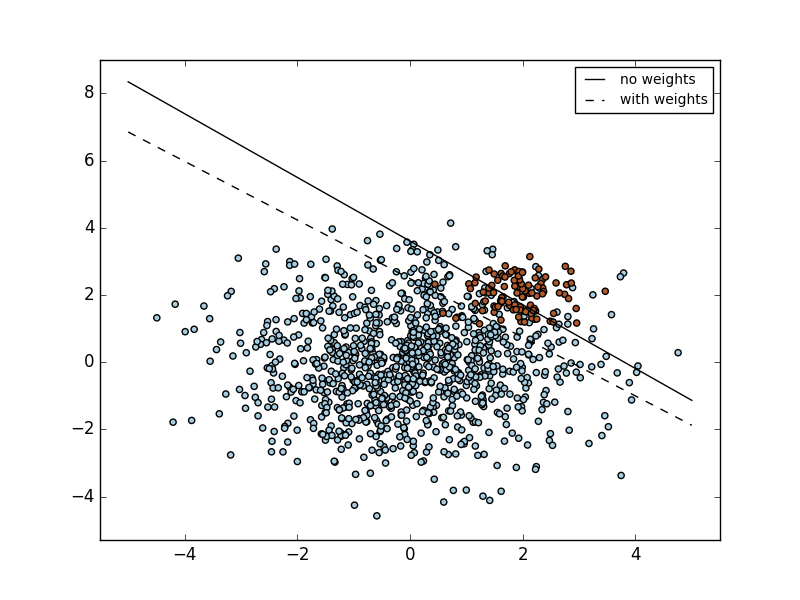
\includegraphics[scale=.4]{SVM1.png}
	\caption{Muestra de desbalance de clases en SVM.}
	\label{SVM1}
\end{figure}

\subparagraph{Complejidad\\\\}

Las máquinas de soporte vectorial son herramientas poderosas, pero sus requerimientos de
computación y almacenamiento aumentan rápidamente con el número de vectores de entrenamiento. El kernel de un SVM es un problema de programación cuadrática (QP), separando los vectores de soporte del resto de los datos de entrenamiento. Es posible eslacar esta solución entre $ O(n_{features} \times n_{samples}^2)$ y $O(n_{features} \times n_{samples}^3)$.

\subparagraph{Formulación Matemática\\\\}

SVM construye un hiperplano o conjunto de hiperplanos en un espacio dimensional alto o infinito, que puede usarse para clasificación, regresión u otras tareas.
Intuitivamente, se logra una buena separación por el hiperplano que tiene la mayor distancia a los
puntos de datos de entrenamiento más próximos de cualquier clase (llamado margen funcional), ya
que en general, cuanto mayor es el margen, menor es el error de generalización del clasificador, tal como se expone en la Figura  \ref{SVM2}:

\begin{figure}[!h]
	\centering
	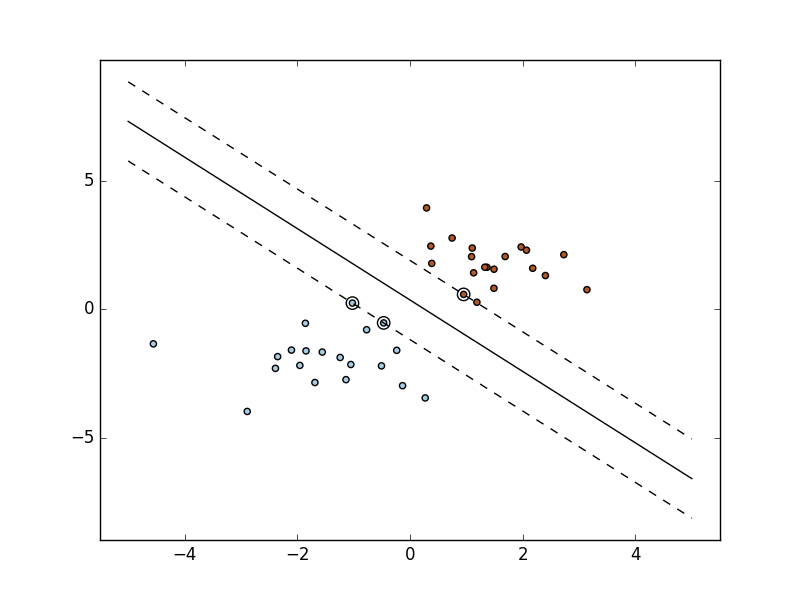
\includegraphics[scale=.4]{SVM2.png}
	\caption{Esquema de hiperplanos en SVM.}
	\label{SVM2}
	
\end{figure}

Se expone la formulación matemática para cada uno de los clasificadores expuestos anteriormente:

\subparagraph{SVC\\\\}

Dado los vectores de entrenamiento $x_{i}\ \in\ R$,
 i=1,..., n, en dos clases, y un vector, $y \in \{1, -1\}^n$, SVC resuelve el siguiente problema primario:

\begin{center}
	$\min_ {w, b, \zeta} \frac{1}{2} w^T w + C \sum_{i=1}^{n} \zeta_i$
\end{center}
\begin{center}
	
	$para\ la\ clase\ y_i (w^T \phi (x_i) + b) \geq 1 - \zeta_i,\ \zeta_i \geq 0, i=1, ..., n$	
\end{center}

Su doble es

\begin{center}
	$\min_{\alpha} \frac{1}{2} \alpha^T Q \alpha - e^T \alpha$
\end{center}
\begin{center}
	$para\ la\ clase\ y^T \alpha = 0\ 0 \leq \alpha_i \leq C, i=1, ..., n$
\end{center}

Donde $e$ es el vector de todos los unos, $C > 0$ es el límite superior, $Q$ es una matriz de $n\ x\ n$ definida semipositiva, $Q_{ij} \equiv y_i y_j K(x_i, x_j)$, donde $K(x_i, x_j) = \phi (x_i)^T \phi (x_j)$ es el kernel. Los vectores de entrenamiento son implícitamente mapeados en un espacio dimensional mayor (tal vez infinito) por la función $\phi$.

La función de decisión es:

\begin{center}
	$sgn(\sum_{i=1}^n y_i \alpha_i K(x_i, x) + \rho)$
\end{center}

\subparagraph{NuSVC\\\\}

Se introduce el parámetro $\nu$ el cual controla el número de vectores de soporte y errores de
entrenamiento. El parámetro $\nu \in (0, 1]$ es un límite superior en la fracción de errores de
entrenamiento y un límite inferior de la fracción de vectores de soporte.

\subparagraph{SVR\\\\}

Dados los vectores de entrenamiento  $x_{i} \in\ R^n$  
$\varepsilon-SVR$ \cite{smola2004tutorial} resuelve el siguiente problema primario:

\begin{center}
	
	$\min_ {w, b, \zeta, \zeta^*} \frac{1}{2} w^T w + C \sum_{i=1}^{n} (\zeta_i + \zeta_i^*)
	$
\end{center}

\begin{center}
	
	$para la clase y_i - w^T \phi (x_i) - b \leq \varepsilon + \zeta_i,$
\end{center}
\begin{center}
	$w^T \phi (x_i) + b - y_i \leq \varepsilon + \zeta_i^*,\ \zeta_i, \zeta_i^* \geq 0, i=1, ..., n$	
\end{center}

Donde $e$ es el vector para todos, $C >$ 0 es el límite superior, $Q$ es una matriz de $n\ x\ n$ definida semipositiva, $Q_{ij} \equiv K(x_i, x_j) = \phi (x_i)^T \phi (x_j)$ es el kernel. Aquí los vectores de
entrenamiento son implícitamente mapeados en un espacio dimensional mayor (tal vez infinito) por
la función $\phi$.

La función de decisión es:

\begin{center}
	$\sum_{i=1}^n (\alpha_i - \alpha_i^*) K(x_i, x) + \rho$
\end{center}

\subsection{Métodos de ensamble}

Los métodos de ensamble, se basan en la combinación de las predicciones obtenidas por varios estimadores construidos en base a algoritmos de aprendizaje supervisado, con el fin de mejorar la generalización del modelo y aumentar la robustez ante nuevos ejemplos \cite{dietterich2000ensemble}.

Existen dos familias de métodos de ensamble, las cuales se diferencian principalmente en la forma en que combinan los modelos para obtener la medida de desempeño final \cite{kotsiantis2007supervised}:

\begin{enumerate}
	
	\item Métodos ponderado, basados en la construcción de varios estimadores independientes y promediar sus medidas de desempeño, esto mejora el rendimiento debido a que disminuye la variabilidad de las clasificaciones. Ejemplos comunes de esto son Bagging, Random Forest.
	
	\item Métodos boosting: basados en la construcción secuencial de modelos, intentando disminuir el sesgo del modelo combinando, cumple con la filosofía \textit{"la unión de varios modelos débiles, puede construir uno fuerte"}. Ejemplos comunes de esto son AdaBoost, Gradient Tree Boosting.
	
\end{enumerate}

A continuación se explican brevemente algunos de los algoritmos asociados a la familia de métodos de ensamble.

\subsubsection{Bagging}

Bagging forma parte de los métodos ponderados, en particular, se puede definir como métodos que forman una clase de algoritmos compuestos por varias instancias de un estimador, entrenados en base a subconjuntos aleatorios del set de datos original, ponderando sus predicciones individuales en una respuesta ponderada. El objetivo general de estos métodos es reducir la varianza de un estimador, por medio del proceso de entrenamiento de subconjuntos aleatorios \cite{breiman1996bagging}. 

Existen diferentes formas de formar los subconjuntos aleatorios de entrenamiento, dentro de las cuales se destacan las siguientes.

\begin{itemize}
	
	\item Los subconjuntos aleatorios del conjunto de datos se basan en subconjuntos aleatorios de las muestras, esto se conoce como \textit{"Pasting o Pegado"} \cite{breiman1999pasting}. 
	
	\item Las muestras se extraen con reemplazo, siendo este método conocido como \textit{"Bagging"} \cite{breiman1996bagging}.
	
	\item Los subconjuntos aleatorios del conjunto de datos se basan en subconjuntos aleatorios de las características, esto se conoce como \textit{"subespacios aleatorios"} \cite{barandiaran1998random}.
	
	\item Los subconjuntos aleatorios se crean en base a subconjuntos aleatorios de características y muestras, esto se conoce como \textit{"Random Patches"} \cite{ref10.1007/978-3-642-33460-3_28}.
	
\end{itemize}

\subsubsection{Random Forest}

Random Forest es un método de ensamble ponderado basado en árboles de decisión aleatorios. Conjuntos de diversos clasificadores son creados basados en efectos aleatorios tanto de la extracción de características como de ejemplos, formando subconjuntos de elementos, cada uno de estos aporta con un valor de estimación, el cual es ponderado con los restantes, obteniendo así, la medida general \cite{breiman1998}.

Un esquema representativo del proceso, es como se expone en la Figura \ref{rf1}. En ella, se aprecian que se generan $n$ árboles, los cuales contemplan diferentes cantidades de ejemplos o atributos y la estimación final se basa en una ponderación, ya sea por proceso de votación, en el caso de modelos de clasificación, o simplemente por la media, para modelos de regresión \cite{Breiman2001}.

\begin{figure}[!h]
	\centering
	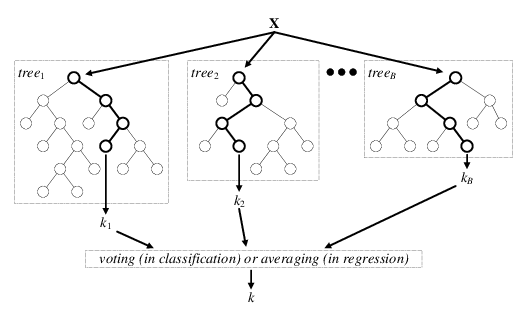
\includegraphics[scale=.5]{rf.png}
	\caption{Esquema representativo de algoritmo Random Forest.}
	\label{rf1}
	
\end{figure}
 
\subsubsection{AdaBoost}

AdaBoost, es un algoritmo basado en el método boosting, lo que implica que se ajusta a una secuencia de estimadores débiles obtenidos a partir de diferentes subconjuntos de datos generados de manera aleatoria desde el conjunto inicial de datos de entrenamiento \cite{CAO2013745}. Cada una de las predicciones obtenidas por los estimadores se combinan de manera ponderada por votación, en el caso de modelos de clasificación, o a través de un promedio en base a las estimaciones resultantes, en el caso de modelos de regresión.

Las modificaciones de los datos en cada iteración de boosting, consisten en aplicar pesos $w_{1},w_{2},..,w_{N}$, a cada una de las muestras de entrenamiento. Inicialmente, todos los pesos están configurados en $\Psi_{i}\ =\ 1/N$, de modo que el primer paso simplemente entrena un modelo débil en los datos originales. Para cada iteración sucesiva, las ponderaciones de la muestra se modifican individualmente y el algoritmo de aprendizaje se vuelve a aplicar a los datos ponderados. En un paso dado, los ejemplos de entrenamiento que fueron predichos incorrectamente por el modelo mejorado inducido en el paso anterior tienen sus pesos incrementados, mientras que los pesos se disminuyen para aquellos que fueron predichos correctamente \cite{hastie2009multi}. A medida que avanzan las iteraciones, los ejemplos que son difíciles de predecir reciben una influencia cada vez mayor. Por lo tanto, cada modelo de aprendizaje débil subsiguiente se ve forzado a concentrarse en los ejemplos que se pierden en los anteriores en la secuencia.

\subsubsection{Gradient Tree Boosting}

Gradient Tree Boosting o Gradient Boosted Regression Trees, es una generalización de métodos de boosting para funciones diferenciables arbitrarias de pérdida \cite{gradient}. Es un método considerado como preciso y efectivo, el cual puede usarse tanto para el desarrollo de modelos de clasificación como de regresión, siendo usado en diferentes áreas de investigación: motores de búsqueda, ecología, minerología, biotecnología, entre otros.

Dentro de las principales ventajas que posee se encuentran: manejo natural de diferentes tipos de características en un set de datos, alto poder predictivo y robusto frente a la predicción de valores atípicos en una muestra \cite{FRIEDMAN2002367}.
 
\subsection{Redes Neuronales y Deep Learning}

Redes neuronales es posible definirlas como una serie de modelos de aprendizaje que se basan en la forma de trabajo de las redes neuronales biológicas, es decir, se usa el concepto de \textit{neurona} para estimar una función aproximada, la cual dependerá de un largo número de inputs, generalmente desconocidos.

En la imagen \ref{red} se aprecia un sistema de red neuronal, en la cual se observa un sistema interconectado por neuronas, las cuales intercambian información en forma de mensaje entre ellas, además cada interconexión tiene un peso, el cual es un valor numérico, que puede ser obtenido en base a la experiencia, en resumen, una red neuronal es un conjunto de entradas y salidas regidas por capas intermedias que permiten evaluar la salida, dichas capas operan entre sí en base a funciones matemáticas y brindan un peso a la conexión, finalmente cada capa es usada para diseñar un modelo de aprendizaje supervisado o no.

\begin{figure}[!h]
	\centering
	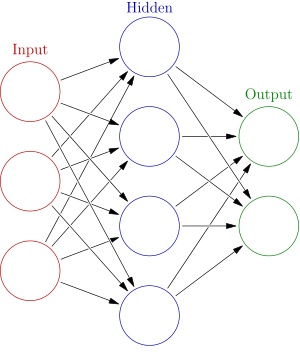
\includegraphics[scale=.45]{red.png}
	\caption{Representación esquemática de una Red Neuronal}
	\label{red}
\end{figure} 

Deep Learning es una herramienta de Machine Learning la cual tiene por objetivo modelar abstracciones de alto nivel en los datos por medio del uso de múltiples capas de procesamiento, ya sea a través del uso de estructuras complejas a través de múltiples transformaciones no lineales \cite{bengio2013representation, MAL-006, SIG-039}. 

La investigación en esta área tiene por objetivo generar mejores representaciones y crear modelos para aprender de éstas a partir de datos no marcados a gran escala. En geneal, las representaciones obtenidas se inspiran en los avances en la neurociencia y se basa libremente en la interpretación de los patrones de procesamiento y comunicación de información en un sistema nervioso, como la codificación neural que intenta definir una relación entre varios estímulos y respuestas neuronales asociadas en el cerebro \cite{MAL-006}.

Deep learning es un método específico de machine learning el cual incorpora redes neuronales organizadas en capas consecutivas para poder aprender iterativamente utilizando un conjunto de datos. Deep learning es especialmente útil cuando se desea aprender patrones provenientes de datos no estructurados \cite{SIG-039}.

Posee diversas arquitecturas, tales como: deep learning network, matrices de convoluciones, redes neuronales recurrentes, etc. las cuales han sido utilizadas en visión artificial para el reconocimiento de patrones, aprendizaje de escritura, etc. Deep Learning es una herramienta de Machine Learning la cual tiene por objetivo modelar abstracciones alto nivel en los datos por medio del uso de múltiples capas de procesamiento, ya sea a través del uso de estructuras complejas a través de múltiples transformaciones no lineales \cite{arel2010deep}.

Dentro de los principales algoritmos que son utilizados en redes neuronales se encuentran Back Propagation \cite{HECHTNIELSEN199265} y Multi Layer Perceptron \cite{80266}.

\subsection{Medidas de desempeño}

Medir el desempeño del modelo predictivo es importante a la hora de evaluar qué tan efectivo es el entrenamiento y la clasificación que se genera, existen medidas que sólo se basan en la cantidad de aciertos o errores que comete el clasificador, otras que implican la eficiencia del modelo y otras que se basan en la precisión, se define brevemente algunas de las medidas más utilizadas a la hora de evaluar modelos de aprendizaje supervisados:

\begin{itemize}
	
	\item \textbf{Tasa de Verdaderos Positivos}: corresponde a la medida asociada a las correctas clasificaciones versus el total de clasificaciones realizadas, es decir, cuántos predicciones efectivas se obtuvieron con respecto a una clase.
	
	\item \textbf{Tasa de Falsos Positivos}: corresponde a la medida asociada a las clasificaciones mal efectuadas, es decir, cuántas predicciones erradas existen con respecto a una clase.
	

	\item \textbf{Accuracy}: corresponde al total de predicciones correctas con respecto al total de la muestra. Sea $\hat{y}_i$ el valor de predicción del ejemplo $i$ e $y_{i}$ corresponde al verdadero valor, la Accuracy se define como: $\texttt{accuracy}(y, \hat{y}) = \frac{1}{n_\text{samples}} \sum_{i=0}^{n_\text{samples}-1} 1(\hat{y}_i = y_i)$
	
	\item \textbf{Precision}: es la capacidad del clasificador para no etiquetar como positiva una muestra que es negativa, se define como: $\text{precision} = \frac{tp}{tp + fp}$, donde tp corresponde a verdaderos positivos y fp a los falsos positivos.
	
	
	\item \textbf{Recall}: es la capacidad del clasificador para encontrar todas las muestras positivas, se define como: $\text{recall} = \frac{tp}{tp + fn}$ , donde tp corresponde a verdaderos positivos y fp a los falsos positivos.
	
	\item \textbf{F-$\beta$}: representa una ponderación armónica entre la Precision y el Recall, se define como: $F_\beta = (1 + \beta^2) \frac{\text{precision} \times \text{recall}}{\beta^2 \text{precision} + \text{recall}}.$ , donde tp corresponde a verdaderos positivos y fp a los falsos positivos y $\beta$ un factor de ponderación.
	
	\item \textbf{Coeficiente de correlación de Matthews}: Se asocia a una medida de la calidad de las clasificaciones, la cual no se ve afectada por el desbalance de clases que pudiese existir, se define como $MCC = \frac{tp \times tn - fp \times fn}{\sqrt{(tp + fp)(tp + fn)(tn + fp)(tn + fn)}}$, donde tp corresponde a verdaderos positivos y fp a los falsos positivos.
		
\end{itemize}

Las mediciones expuestas previamente, se utilizan para medir el desempeño de modelos de clasificación, mientras que para evaluar un estimador basado en respuestas continuas, normalmente se utilizan las siguientes:

\begin{itemize}
	
	\item \textbf{Coeficiente de Pearson}: Medida lineal entre dos variables cuantitativas aleatorias que permite evaluar el grado de relación entre ellas, se encuentra en rangos entre -1 y 1 donde -1 indica que las variables no presentan relación y 1 que las muestras están estrechamente relacionadas. Se obtiene a partir de $\rho X,Y= \frac{n\sum x_{i}y_{i} - \sum x_{i} \sum y_{i}}{\sqrt{n\sum x^{2}_{i}- (\sum x_{i})^{2}} \sqrt{n\sum y^{2}_{i}- (\sum y_{i})^{2}}}$ donde $x_{i}$ representa los valores de predicción e $y_{i}$ representa los valores reales de la muestra para $n$ ejemplos.
	
	\item \textbf{Coeficiente de Spearman}: Medida de correlación que permite evaluar la asociación o relación entre dos muestras, su interpretación es similar al coeficiente de Pearson y se estima a partir de $\rho = 1- \frac{6\sum D^{2}}{N(N^{2}-1)}$ donde $D$ es la diferencia $x-y$ para el $i-th$ ejemplo y $N$ es el total de ejemplos en la muestra.
	
	\item \textbf{Kendall $\tau$ rank}: Medida que permite evaluar la relación entre dos variables, su interpretación es similar a las basadas en coeficiente de Pearson y Spearman. Se obtiene a partir de $\tau = \frac{\text{(numbers of concordant pairs)} - \text{(number of discordant pairs)}}{n(n-1)/2}$
	
	\item \textbf{Coeficiente de determinación $R^{2}\ score$}: es una medida que cuantifica cómo el predictor se adapta a nuevos ejemplos, posee un rango entre -1 y 1 donde -1 es lo peor y 1 lo mejor, esto es debido a que el estimador puede bajar su rendimiento. Se estima en base a $R^2(y, \hat{y}) = 1 - \frac{\sum_{i=0}^{n_{\text{samples}} - 1} (y_i - \hat{y}_i)^2}{\sum_{i=0}^{n_\text{samples} - 1} (y_i - \bar{y})^2}$ donde $\hat{y}_i$ corresponde al valor predicho para el $i-th$ ejemplo e $y_{i}$ corresponde al valor real en una muestra de $n-samples$.
	
	\item \textbf{Error medio absoluto}: Estima la diferencia positiva entre el valor real y el valor predicho para un conjunto de ejemplos. Se estima a partir de $\text{MAE}(y, \hat{y}) = \frac{1}{n_{\text{samples}}} \sum_{i=0}^{n_{\text{samples}}-1} \left| y_i - \hat{y}_i \right|.$ donde $\hat{y}_i$ corresponde al valor predicho para el $i-th$ ejemplo e $y_{i}$ corresponde al valor real en una muestra de $n-samples$.
	
	\item \textbf{Error cuadrático medio}: Estima la diferencia cuadrática entre el valor real y el valor predicho para un conjunto de ejemplos. Se obtiene a partir de $\text{MSE}(y, \hat{y}) = \frac{1}{n_\text{samples}} \sum_{i=0}^{n_\text{samples} - 1} (y_i - \hat{y}_i)^2$ donde $\hat{y}_i$ corresponde al valor predicho para el $i-th$ ejemplo e $y_{i}$ corresponde al valor real en una muestra de $n-samples$.
	
	\item \textbf{Error logarítmico cuadrático medio}: Es similar al error cuadrático medio, la diferencia principal es que se utiliza el logaritmo natural de las diferencias entre respuesta y valor predicho. Se estima en base a $\text{MSLE}(y, \hat{y}) = \frac{1}{n_\text{samples}} \sum_{i=0}^{n_\text{samples} - 1} (\log_e (1 + y_i) - \log_e (1 + \hat{y}_i) )^2$ donde $\hat{y}_i$ corresponde al valor predicho para el $i-th$ ejemplo e $y_{i}$ corresponde al valor real en una muestra de $n-samples$.
	
	\item \textbf{Error mediano absoluto}: es una medida robusta ante outliers, la pérdida o el error se calcula a partir de las medianas de las diferencias absolutas entre la respuesta y el valor predicho. Se estima en base a $\text{MedAE}(y, \hat{y}) = \text{median}(\mid y_1 - \hat{y}_1 \mid, \ldots, \mid y_n - \hat{y}_n \mid)$ donde $\hat{y}_i$ corresponde al valor predicho para el $i-th$ ejemplo e $y_{i}$ corresponde al valor real en una muestra de $n-samples$.
	  
	
\end{itemize}

\subsection{Problemas asociados a los modelos de aprendizaje supervisado}

Dentro de los principales problemas que pueden presentar los modelos de aprendizaje supervisado se encuentran las situaciones en las que la cantidad de atributos que puede contener un set de datos es mucho mayor con respecto a la cantidad de ejemplos que se posee, conocido también como \textit{"Maldición de la dimensionalidad"} \cite{indyk1998approximate}, es decir si existen $n$ ejemplos y la cantidad de atributos es $n\ x\ n$ es posible que ocurra dicha problemática, para solucionar este problema, existen técnicas asociadas a reducción de dimensionalidad \cite{sarwar2000application, van2009dimensionality}, siendo las más utilizadas métodos lineales de reducción como PCA y derivados, Análisis de características basados en modelos de clasificación/regresión aplicando Random Forest, técnicas probabilísticas asociadas al Mutual Information y evaluación de características relacionadas mediante coeficientes de Pearson o matrices de Correlación\footnote{Estas técnicas, se explican en el capítulo \textit{\textbf{Digitalizando propiedades fisicoquímicas de proteínas a partir de su secuencia lineal}}}. En forma similar, también existe que un set de datos contemple una gran cantidad de ejemplos y sus descriptores sean escasos. Estos casos se tratan con técnicas de reducción de dimensionalidad y contemplan la eliminación de ejemplos redundantes con el fin de maximizar la variabilidad de los ejemplo, técnicas como Mutual Information, Análisis de Correlaciones son bastante utilizadas en este problema. Otro posible problema que se puede denotar es el sobreajuste \cite{hawkins2004problem}, esto quiere decir, que el modelo es extremadamente complejo, por lo que éste se ajusta muy bien al set de entrenamiento, no obstante a la hora de probar con nuevos set de datos no representa la performance obtenida. Finalmente, un problema adicional a los modelos de clasificación o regresión se basa en el desbalance de clases o en la tendencia hacia rangos específicos de valores en métodos de regresión \cite{japkowicz2002class}. Esto quiere decir, que existe una diferencia significativa entre los contadores de categorías asociadas a las clases, lo cual afecta a los algoritmos a la hora de entrenar, debido a que aumenta el riesgo de cometer errores del tipo falso positivo. Normalmente, esto conlleva a una reducción de ejemplos de la clase mayoritaria en la etapa de entrenamiento o si es posible, la adición de nuevos ejemplos de la clase minoritaria. 


\subsection{Validación de modelos}

La validación de los modelos trata los problemas de sobreajuste y la generalización, es decir, evitar desarrollar modelos que sólo tengan buenas métricas o medidas de desempeño para los datos de entrenamiento y no permitan clasificar nuevos ejemplos. Con el fin de poder evitar esta problemática, normalmente los set de datos se dividen en 3 conjuntos: Entrenamiento, validación y testeo. Esto quiere decir, se considera una porción de elementos para entrenar el modelo, una segunda instancia para obtener las medidas de desempeño y una tercera con el fin de determinar si el clasificador entrega resultados acorde a las respuestas conocidas. Sin embargo, existen técnicas que a partir del set de entrenamiento, generan múltiples divisiones, con el fin de entrenar subconjuntos de elementos del conjunto de entrenamiento y así obtener modelos ponderados, esto permite aumentar la generalización del modelo, debido a que las medidas de desempeño varían de levemente de aplicación en aplicación y al considerar dicha técnicas, se tienen distribuciones de las medidas del modelo, reportando siempre, la media de dicha distribución. Dentro de las principales técnicas de validación se encuentra la Validación cruzada con $k$ divisiones y un caso particular conocido como \textit{Leave one out}, en el cual el valor de $k$ es igual a la cantidad de ejemplos en el entrenamiento. Éstas se explican a continuación.

\subsubsection{Validación Cruzada}

La validación cruzada, a veces llamada estimación de la rotación, es una técnica de validación del
modelo para evaluar cómo los resultados de un análisis estadístico se generalizarán a un conjunto de datos independiente. Se utiliza principalmente en entornos donde la meta es la predicción, y se
quiere estimar la precisión con la que un modelo predictivo se llevará a cabo en la práctica \cite{crossval}. En un
problema de predicción, a un modelo se le suele asignar un conjunto de datos, de los datos conocidos sobre los que se ejecuta el entrenamiento (conjunto de datos de formación) y un conjunto de datos desconocidos (o primeros datos) contra los que se prueba el modelo. El objetivo de la validación cruzada es definir un conjunto de datos para \textit{probar} el modelo en la fase de entrenamiento (es decir, el conjunto de datos de validación), con el fin de limitar problemas como sobre ajuste.

La idea es dividir el set de datos totales abarcando un set de entrenamiento y un set de validación, lo cual se puede explicar en la Figura  \ref{VC}:

\begin{figure}[!h]
	\centering
	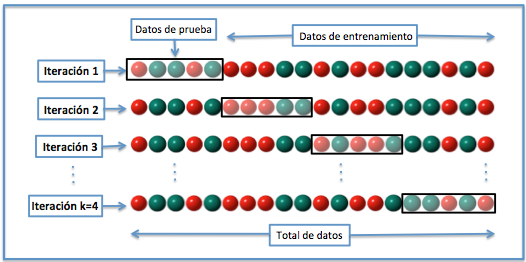
\includegraphics[scale=.5]{validacionCruzada.jpg}
	\caption{Esquema representativo de validación cruzada.}
	\label{VC}
\end{figure}

Una ronda de validación cruzada implica dividir una muestra de datos en subconjuntos complementarios, realizar el análisis en un subconjunto (denominado conjunto de entrenamiento) y
validar el análisis en el otro subconjunto (denominado conjunto de validación o conjunto de pruebas). Para reducir la variabilidad, varias rondas de validación cruzada se realizan utilizando diferentes particiones, y los resultados de validación se promedian durante las rondas, siendo las más utilizadas \textit{10-fold cross validation}.

\subsubsection{Leave one out (Dejar uno)}

Es un tipo especial de validación cruzada, en donde se tiene una muestra con $n$ ejemplos en la etapa de entrenamiento se subdivide dicho set de datos considerando $n-1$ elementos, de tal manera que 1 no se considera, la idea en particular radica en entrenar con los $n-1$ ejemplos y validar o testear con el ejemplo restante, esto se itera $n$ veces, tal como se expone en \ref{LOO}, implicando una mayor cantidad de iteraciones que validación cruzada, provocando además un mayor coste computacional \cite{kohavi1995study}.

\begin{figure}[!h]
	\centering
	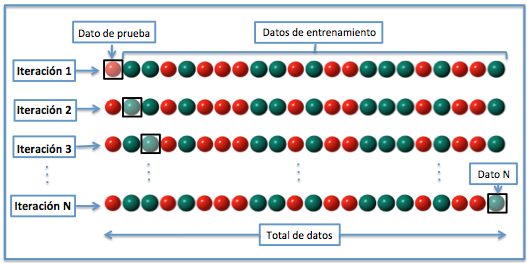
\includegraphics[scale=.5]{Leave-one-out.jpg}
	\caption{Esquema representativo de Leave One.}
	\label{LOO}
\end{figure}


\subsection{Meta Learning}


\section{Hipótesis}

En base a las herramientas existentes y en vista del aumento considerable de datos asociados a mutaciones en proteínas y el conocimiento de las respuestas que éstas generan, se evidencia la necesidad del desarrollo de herramientas computacionales o nuevos modelos de clasificación o regresión que faciliten el entrenamiento de proteínas singulares y la evaluación de sus mutaciones puntuales, con el fin de poder evaluar nuevos ejemplos y cuáles serían los efectos de estos, sin tener que entrar en grandes costos económicos y tiempos de espera. 

Dado esto se propone la siguiente hipótesis.\\

\textit{Es posible utilizar técnicas de Meta Learning y algoritmos de aprendizaje supervisado para la generación de modelos de clasificación o regresión de mutaciones puntuales descritas a partir de sus propiedades termodinámicas y filogenéticas?}\\

Además de la hipótesis central surgen interrogantes como.

\begin{itemize}
	
	\item Es posible utilizar estos nuevos modelos como herramientas para diagnóstico médico?
	\item Cómo se evalúan la robustez y la generalización de estos modelos, serán capaces de adaptarse a nuevos ejemplos?
	\item Es factible el desarrollo de una herramienta computacional que permita entrenar diferentes set de datos y que facilite la clasificación de nuevos ejemplos?
	
\end{itemize}

\section{Objetivos}

En base a la hipótesis planteada y a las preguntas adicionales expuestas, se exponen a continuación el objetivo general y los objetivos específicos.

\subsection{Objetivo general}

Diseñar e implementar estrategias de Meta Learning para la implementación de modelos de clasificación y regresión asociado a mutaciones puntuales en proteínas de interés basados en descriptores termodinámicos, estructurales y filogenéticos.

\subsection{Objetivos específicos}

Dentro de los objetivos específicos se encuentran los siguientes.

\begin{enumerate}
	
	\item Preparar y describir, por medio de propiedades termodinámicas, estructurales y filogenéticas, set de datos de mutaciones puntuales de proteínas con respuesta conocida expuestos en bibliografía o bases de datos reconocidas.
	
	\item Implementar y evaluar metodología de meta learning para el diseño de meta modelos de clasificación y regresión de mutaciones puntuales aplicados a set de datos de proteínas generadas.
	
	\item Diseñar e implementar herramienta computacional que permita el entrenamiento de set de datos y el uso de meta modelos para la evaluación de nuevos ejemplos.
	
	\item Testear y evaluar comportamiento de la herramienta y los meta modelos en base a sistemas de datos que involucren mutaciones en proteínas con respuesta conocida.
	
	\item Implementar modelos de clasificación para la relevancia clínica de mutaciones puntuales en proteína pVHL, asociada a la enfermedad von Hippel Lindau. 
	
\end{enumerate}

\section{Metodología propuesta}

Con el fin de poder responder hipótesis planteada y dar solución a los objetivos, se propone una metodología general en la cual se consideran diferentes estrategias, implementaciones y evaluación de modelos. A continuación se explica la metodología general propuesta y los componentes principales de ésta.

\subsection{Preparación de set de datos}

La preparación del set de datos consiste en obtener data para poder entrenar los modelos de clasificación, la data se asocia a información de mutaciones en proteínas y la respuesta que ésta genera. En la Figura \ref{C2:M1} se expone un esquema general con los pasos desarrollados para la preparación del set de datos.

\begin{figure}[!h]
	\centering
	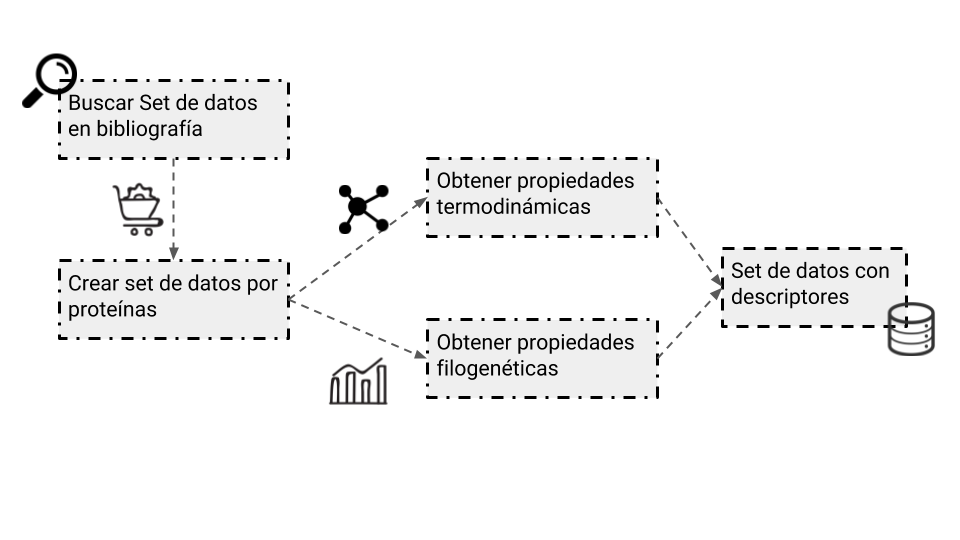
\includegraphics[scale=.4]{m1.png}
	\caption{Esquema representativo asociado al proceso de generación de set de datos de mutaciones puntuales en proteínas.}
	\label{C2:M1}
\end{figure}

Tal como se expone en la Figura \ref{C2:M1}, los set de datos se buscan en la bibliografía, a partir de modelos desarrollados previamente, bases de datos en la literatura, etc. El objetivo fundamental, es encontrar proteínas con mutaciones puntuales cuyo efecto sea conocido, dicha respuesta puede ser categórica, es decir, asociada al diseño e implementación de modelos de clasificación o continua y se aplica para modelos de regresión. 

En una segunda instancia, a partir de la data recolectada ésta se procesa con el fin de poder obtener set de datos de proteínas individuales con una cantidad de ejemplos considerables que permitan el diseño de modelos válidos, para ello, scripts fueron implementados bajo el lenguaje de programación Python con el fin de recuperar las proteínas, obtener la información y generar la data de manera individual, además, eliminar ejemplos ambiguos. Es decir, filas con los mismos valores pero cuya columna de respuesta fuese diferente. 

A partir de esto se forman $n$ set de datos asociados a $n$ proteínas, cada uno con $m$ ejemplos y cuyos descriptores consisten en el residuo original, posición en proteína, residuo mutado y la respuesta asociada. El desbalance de clases se analiza con respecto a las posibles categorías existentes en la respuesta y el porcentaje de representatividad que éstas poseen en la muestra, eliminando aquellos ejemplos cuyo valor no superara el 5\% del total de ejemplos.

Posteriormente se aplican las herramientas SDM \cite{Pandurangan2017} y MOSST \cite{Olivera-Nappa2011} con el fin de obtener los descriptores asociados a las propiedades termodinámicas y filogenéticas. Para ello, scripts Python son desarrollados para consumir los servicios de dichas herramientas y registrar los resultados obtenidos, formando así set de datos con los descriptores planteados en los objetivos iniciales.

Ya con los descriptores formados, las características asociadas a variables categóricas son codificadas. Si la totalidad de posibles categorías supera el 20\% del total de características en el set de datos, se aplica Ordinal Encoder, en caso contrario, One Hot Encoder \cite{pedregosa2011scikit}. Ordinal Encoder consiste en la transformación de variables categóricas en arreglos de números enteros con valores desde $0,...,n-1$ para $n$ posibles categorías. Por otro lado One Hot Encoder, consiste en agregar tantas columnas como posibles categorías existan en el set de datos completadas mediante binarización de elementos (0 si la característica no se presencia, 1 en caso contrario).

Es importante mencionar que las respuestas asociadas a las mutaciones pueden ser del tipo continuo o categórico, lo cual implica que tanto los modelos como las métricas varían. No obstante, se mantiene las respuesta con el fin de demostrar la robustez del método y la eficacia de éste sin importar el tipo de modelo que se éste entrenando.

\subsection{Implementación de meta modelos de clasificación/regresión}

La implementación de meta modelos consiste en la obtención de un grupo de estimadores que en conjunto, permiten clasificar o predecir nuevos ejemplos. Para ello, se diseña e implementa una metodología basada en Meta Learning System y aplicando conceptos similares a los utilizados por los métodos de ensamble en la etapa de evaluación del desempeño del clasificador.

En la Figura \ref{C2:M2}, se exponen las etapas asociadas a la implementación de meta modelos, contemplando desde la fase de entrenamiento de los modelos hasta la unión en meta clasificadores \textbf{Acá debo citar el paper del MLSTraining Tool :D}. Cada una de las etapas contempla un conjunto de scripts implementados en lenguaje de programación Python y empleando la librería Scikit-Learn para el entrenamiento y evaluación de los clasificadores o predictores \cite{pedregosa2011scikit}.


\begin{figure}[!h]
	\centering
	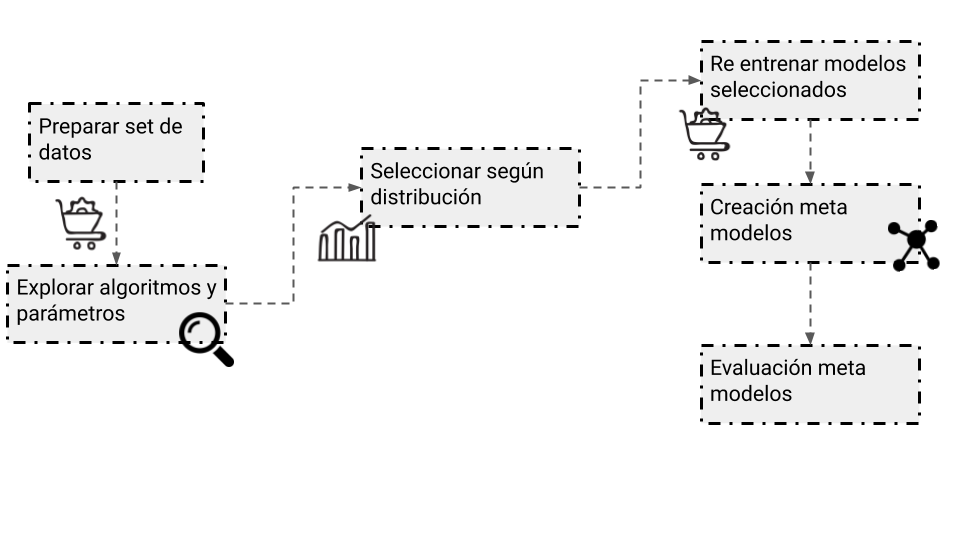
\includegraphics[scale=.4]{m2.png}
	\caption{Esquema representativo asociado al proceso de creación de meta modelos utilizando Meta Learning System Tools.}
	\label{C2:M2}
\end{figure}

Tal como se observa en la Figura \ref{C2:M2}, es posible identificar etapas claves en el proceso: Exploración de modelos, Selección y Generación de los meta clasificadores/predictores. Cada una de estas etapas se exponen a continuación.

\subsubsection{Exploración de modelos}

La exploración de modelos o estimadores, se basa en la aplicación de diferentes algoritmos de aprendizaje supervisado con variaciones en sus parámetros de configuración inicial. La utilización de los algoritmos, depende principalmente del tipo de respuesta que presente el set de datos, es decir, si es continua o categórica. No obstante, a modo resumen, en la Tabla \ref{cap2:tab1} se exponen los algoritmos utilizados, el caso en el que se usan y los parámetros que se varían junto con el total de iteraciones posibles para cada elemento:

\begin{longtable}[c]{llll|l|l|}
	\hline
	\multicolumn{6}{|c|}{\textbf{Algoritmos y parámetros empleados en la etapa de Exploración en MLSTraining}}                                                                                                                                                                                                                                                                                               \\ \hline
	\endfirsthead
	%
	\endhead
	%
	\multicolumn{1}{|l|}{\textbf{\#}} & \multicolumn{1}{l|}{\textbf{Algoritmo}}                                                  & \multicolumn{1}{l|}{\textbf{Tipo}}    & \textbf{Parámetros}                                                                                                                 & \textbf{Uso}                                                         & \textbf{Iteraciones} \\ \hline
	\multicolumn{1}{|l|}{1.}          & \multicolumn{1}{l|}{Adaboost}                                                            & \multicolumn{1}{l|}{Ensamble}         & \begin{tabular}[c]{@{}l@{}}Algoritmo\\ Número estimadores\end{tabular}                                                              & \begin{tabular}[c]{@{}l@{}}Clasificación \\ y Regresión\end{tabular} & 16                   \\ \hline
	\multicolumn{1}{|l|}{2.}          & \multicolumn{1}{l|}{Bagging}                                                             & \multicolumn{1}{l|}{Ensamble}         & \begin{tabular}[c]{@{}l@{}}Bootstrap\\ Número estimadores\end{tabular}                                                              & \begin{tabular}[c]{@{}l@{}}Clasificación y\\ Regresión\end{tabular}  & 16                   \\ \hline
	\multicolumn{1}{|l|}{3.}          & \multicolumn{1}{l|}{\begin{tabular}[c]{@{}l@{}}Bernoulli\\ Naive Bayes\end{tabular}}     & \multicolumn{1}{l|}{Probabilístico}   & Default                                                                                                                             & Clasificación                                                        & 1                    \\ \hline
	\multicolumn{1}{|l|}{4.}          & \multicolumn{1}{l|}{Decision Tree}                                                       & \multicolumn{1}{l|}{Características}  & \begin{tabular}[c]{@{}l@{}}Criterio división\\ Función de impureza\end{tabular}                                                     & \begin{tabular}[c]{@{}l@{}}Clasificación y\\ Regresión\end{tabular}  & 4                    \\ \hline
	\multicolumn{1}{|l|}{5.}          & \multicolumn{1}{l|}{\begin{tabular}[c]{@{}l@{}}Gaussian\\ Naive Bayes\end{tabular}}      & \multicolumn{1}{l|}{Ensamble}         & Default                                                                                                                             & \begin{tabular}[c]{@{}l@{}}Clasificación y\\ Regresión\end{tabular}  & 1                    \\ \hline
	\multicolumn{1}{|l|}{6.}          & \multicolumn{1}{l|}{\begin{tabular}[c]{@{}l@{}}Gradient\\ Tree Boosting\end{tabular}}    & \multicolumn{1}{l|}{Ensamble}         & \begin{tabular}[c]{@{}l@{}}Función de pérdida\\ Número estimadores\end{tabular}                                                     & \begin{tabular}[c]{@{}l@{}}Clasificación y\\ Regresión\end{tabular}  & 16                   \\ \hline
	\multicolumn{1}{|l|}{7.}          & \multicolumn{1}{l|}{\begin{tabular}[c]{@{}l@{}}k-Nearest\\ Neighbors\end{tabular}}       & \multicolumn{1}{l|}{Distancias}       & \begin{tabular}[c]{@{}l@{}}Número Vecinos\\ Algoritmo\\ Métrica distanciaPesos\end{tabular}                                         & \begin{tabular}[c]{@{}l@{}}Clasificación y\\ Regresión\end{tabular}  & 160                  \\ \hline
	\multicolumn{1}{|l|}{8.}          & \multicolumn{1}{l|}{\begin{tabular}[c]{@{}l@{}}Multi layer\\ perceptron\end{tabular}}    & \multicolumn{1}{l|}{Redes neuronales} & \begin{tabular}[c]{@{}l@{}}Función de activación\\ Solver\\ Taza de aprendizaje\\ Alpha\\ Shuffle\\ Máximo iteraciones\end{tabular} & \begin{tabular}[c]{@{}l@{}}Clasificación y\\ Regresión\end{tabular}  & 2160                 \\ \hline
	\multicolumn{1}{|l|}{9.}          & \multicolumn{1}{l|}{\begin{tabular}[c]{@{}l@{}}Nu Support\\ Vector Machine\end{tabular}} & \multicolumn{1}{l|}{Kernel}           & \begin{tabular}[c]{@{}l@{}}Kernel\\ Nu\\ Grado polinomio\end{tabular}                                                               & \begin{tabular}[c]{@{}l@{}}Clasificación y\\ Regresión\end{tabular}  & 240                  \\ \hline
	\multicolumn{1}{|l|}{10.}         & \multicolumn{1}{l|}{Random Forest}                                                       & \multicolumn{1}{l|}{Ensamble}         & \begin{tabular}[c]{@{}l@{}}Número estimadores\\ Función de impureza\\ Bootstrap\end{tabular}                                        & \begin{tabular}[c]{@{}l@{}}Clasificación y\\ Regresión\end{tabular}  & 32                   \\ \hline
	\multicolumn{1}{|l|}{11.}         & \multicolumn{1}{l|}{\begin{tabular}[c]{@{}l@{}}Support\\ Vector Machine\end{tabular}}    & \multicolumn{1}{l|}{Kernel}           & \begin{tabular}[c]{@{}l@{}}Kernel\\ C\\ Grado polinómio\end{tabular}                                                                & \begin{tabular}[c]{@{}l@{}}Clasificación y\\ Regresión\end{tabular}  & 240                  \\ \hline
	&                                                                                          &                                       &                                                                                                                                     & \textbf{Total Iteraciones}                                           & \textbf{2886}        \\ \cline{5-6} 
	\caption{}
	\label{cap2:tab1}\\
\end{longtable}

Como se observa en la Tabla \ref{cap2:tab1}, son sobre 2800 modelos los que se generan y a partir de ellos se obtiene distribuciones de medidas de desempeño que permiten evaluarlos. En el caso de modelos de regresión se utilizan los coeficientes de Pearson, Spearman, Kendall $\tau$ y $R^{2}$, mientras que para modelos de clasificación, se consideran la Precisión, Exactitud, Recall y F1.

Finalmente esta etapa permite entregar set de modelos entrenados y evaluados según las métricas de interés, se destaca que cada modelo es validado a través del proceso de validación cruzada, considerando un valor $k=10$, con el fin de poder disminuir posibles sobreajustes.

\subsubsection{Selección de modelos}

Cada distribución de medida de desempeño perteneciente los modelos entrenados en la fase de Exploración, se somete a test estadísticos que permite seleccionar los modelos cuyas métricas representen outliers positivos dentro de la distribución.

El algoritmo general, utilizado para el desarrollo de esta selección es como se expone en el algoritmo \ref{alg:select}, para el cual se detallan los pasos simplificados que permiten obtener un conjunto de modelos entrenados y que representan los valores más altos dentro de su distribución. Es importante mencionar que se obtiene un conjunto $M'$ con los modelos, considerando como punto de selecciones los valores evaluados con respecto a la desviación estándar, considerando los cortes 3 $\sigma$, 2 $\sigma$ y 1.5 $\sigma$ por sobre la media, si ningún factor se cumple, sólo se considera el valor máximo en la distribución.

Es importante mencionar, que cada distribución puede permitir la selección de distintos modelos, lo cual implica que un mismo modelo pueda ser seleccionado en diferentes medidas, razón por la cual, a la hora de obtener el conjunto de modelos $M'$ se remueven aquellos elementos que se encuentran repetidos. Siendo estos, sólo los modelos que presenten igualdad tanto en el algoritmo como en sus parámetros de configuración inicial.

\begin{algorithm}[H]
	\begin{algorithmic}[1]
		\REQUIRE Conjunto $M$ con modelos entrenados y sus medidas de desempeño, Lista $L$ con medidas de desempeño. \label{lin:lineaRara}
		\ENSURE Conjunto $M'$ con modelos seleccionados.
		
		
		\FOR{$i$ en $L$} 
		\STATE Calcular  media $\mu$, desviación estándar $\sigma$ en distribución $M_{i}$
		\FOR{$ x \in M_{i}$}
			\IF {$x \ge \mu + 3*\sigma$}
				\STATE Agregar $x$ a $M'$
			\ENDIF
		\ENDFOR
		\IF {largo $M'$ = 0}
			\FOR{$ x \in M_{i}$}
				\IF {$x \ge \mu + 2*\sigma$}
					\STATE Agregar $x$ a $M'$
				\ENDIF
			\ENDFOR
			
			\IF {largo $M'$ = 0}
				\FOR{$ x \in M_{i}$}
					\IF {$x \ge \mu + 1.5*\sigma$}
						\STATE Agregar $x$ a $M'$
					\ENDIF
				\ENDFOR
				
				\IF {largo $M'$ = 0}
					\FOR{$ x \in M_{i}$}
						\IF {$x = MAX{M_{i}}$}
							\STATE Agregar $x$ a $M'$
						\ENDIF
					\ENDFOR
				\ENDIF
			\ENDIF
		\ENDIF
		\ENDFOR
		
		\RETURN $D$ sin valores extremos
	\end{algorithmic}
	\caption{Algoritmo de selección de modelos}\label{alg:select}
\end{algorithm}

\subsubsection{Generación de meta modelos}

A partir del conjunto de modelos $M'$, el cual representa los estimadores seleccionados cuyas medidas de desempeño son las más altas en sus distribuciones correspondientes, se generan meta modelos, es decir, estimadores compuestos de diversas unidades, los cuales en conjunto entregan una respuesta, ya sea por ponderación o votación. El proceso general para la generación de los meta modelos, es descrito a continuación.

En una primera instancia, los modelos son nuevamente entrenados y se comparan las nuevas medidas de desempeño con las obtenidas previamente, en caso de que exista una diferencia mayor al 20\%, en cualquiera de sus métricas, el modelo se remueve del conjunto $M'$. La razón fundamental de esto, es debido a que se espera desarrollar modelos robustos cuyas evaluaciones no presenten variaciones significativas y que realmente no alteren sus predicciones ante nuevos ejemplos, razón por la cual, se aplica nuevamente validación cruzada $k=10$ para validar los modelos.

Con el fin de evaluar el desempeño de los meta clasificadores, nuevas medidas se generan a partir de la información resultante de los modelos individuales. No obstante, la forma en la que se obtienen varían dependiendo del tipo de respuesta que se debe entregar.

Si la respuesta es continua, es decir, los modelos son del tipo regresión, se obtiene los valores de predicción de cada modelo y se promedian, para luego aplicar las métricas estándar (Coeficiente de Pearson, Kendall $\tau$, Spearman y $R^{2}$) sobre estos valores promediados y los reales. 

Para el caso en que la respuesta sea categórica, es decir, los modelos son del tipo clasificación, se obtiene la respuesta de cada modelo individual y se selecciona una única categoría, correspondiente a aquella que presente una mayor probabilidad de ocurrencia dada la distribución de elementos y considerando para ello las probabilidades iniciales de cada categoría en el set de datos de estudio. De esta forma, se obtiene un vector respuesta con la clasificación de cada ejemplo cuyo valor corresponde al evento más probable a ocurrir, este vector se compara con el set de respuestas reales y se aplican las métricas de interés para clasificadores.

\subsection{Cómo usar los meta modelos para la clasificación de nuevos ejemplos?}

Nuevos ejemplos pueden ser clasificados o predecir su respuesta, dependiendo sea el caso, a partir de los meta modelos desarrollados. En el caso de estimadores basados en variables continuas, los nuevos ejemplos se someten a cada uno de los modelos individuales pertenecientes al sistema, los cuales generan una respuesta individual, a partir de dichas respuestas, se genera un intervalo de confianza con un nivel de significancia $\alpha=0.05$ donde existe una mayor probabilidad de que se encuentre el valor real de la predicción. Para ejemplos que impliquen clasificación, se obtiene la respuesta de cada modelo individual y se evalúa la probabilidad de ocurrencia de cada categoría, entregando así, la respuesta condicionada por una probabilidad de ocurrencia del evento.

\subsection{Uso de meta modelos en sistemas de proteínas}

El objetivo principal de esta metodología, radica en el hecho de crear una herramienta que permita implementar modelos basados en algoritmos de aprendizaje supervisado para set de datos de mutaciones puntuales o variantes para una misma proteína. 

Un flujo general del uso de la herramienta, se expone en la Figura \ref{C2:M3}.

\begin{figure}[!h]
	\centering
	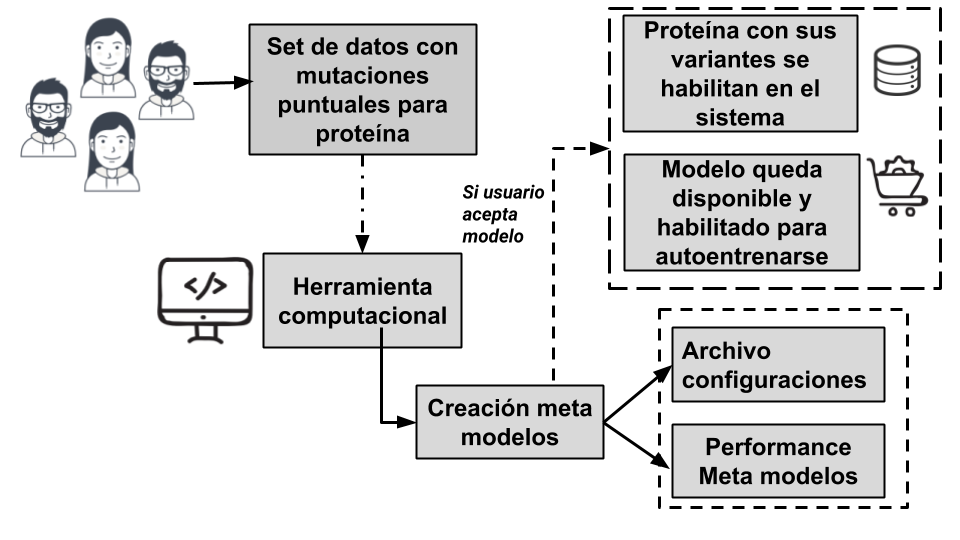
\includegraphics[scale=.4]{m3.png}
	\caption{Esquema representativo de flujo asociado a la herramienta de generación de meta modelos para mutaciones puntuales en proteínas de interés.}
	\label{C2:M3}
\end{figure}

La idea general, consiste en que usuarios de la herramienta, puedan entrenar sus propios modelos de clasificación o regresión, basados en la metodología expuesta en los pasos anteriores mediante el uso de Meta Learning System. Para ello, los usuarios deben entregar sus set de datos con la información necesaria para ser procesada: cadena, residuo original, posición, residuo mutado y respuesta o efecto de la mutación. La herramienta, aplica los pasos expuestos en la metodología de este capítulo generando un meta modelo basado en algoritmos de aprendizaje supervisado y las medidas de desempeño que permiten evaluar el modelo obtenido. Si el usuario acepta la metodología y por medio de un consentimiento informado, permite la publicación de los datos, el sistema habilita el acceso tanto a los meta modelos como a los set de datos y los agrega a la lista de procesos de modelos auto entrenables. Esto último, implica que ante la adición de nuevos ejemplos al set de datos, el sistema actualiza los modelos y las medidas de desempeño, aplicando la metodología expuesta, así, constantemente mantiene la actualización de la información y permite mantener en constante crecimiento los datos que contemplan el desarrollo de los modelos.
 
\section{Resultados y discusión del proceso}

A continuación, se exponen los resultados obtenidos y discusiones a cerca del proceso generado, contemplando desde la etapa inicial asociada a la búsqueda de set de datos de mutaciones en proteínas, la preparación de estos para la aplicación de la metodología desarrollado y la evaluación del funcionamiento de estos con el fin de generar meta modelos asociados a sistemas de mutaciones en proteínas y permitir el desarrollo de herramientas computacionales que faciliten dichas acciones. Adicional a esto, se expone un caso de estudio donde se emplea esta metodología para el desarrollo de modelos de clasificación de relevancia clínica de mutaciones asociadas a la enfermedad de von Hippel-Lindau.

\subsection{Set de datos utilizados}

En el presente apartado se describen las características básicas de los set de datos trabajados, así como también qué representan las proteínas bajo las cuales se están desarrollando los modelos de estimadores.

\subsubsection{Descripción general}

Los set de datos utilizados, tanto para la formación de los inputs asociados al sistema, así como también la validación de respuesta correspondiente a la mutación que estos tienen, fueron extraídos desde distintas bases de datos de mutaciones en proteínas de estudios relacionados a los cambios que provoca la sustitución del residuo inicial, ya sea a nivel de cambios energéticos o estabilidad de la proteína, obteniendo 11 set de datos de mutaciones con respuesta continua basada en diferencias de energía libre de Gibbs, cuyos reportes se centran en \cite{Wainreb2011, Sun2017, petukh2016saambe, Alexov2012,prot20185}, mientras que 8 set de datos corresponden a set del tipo clasificación \cite{ancien2018prediction, broom2017computational, capriotti2008three, quan2016strum, Capriotti2005, 1gzp030, Khan2010, masso2008accurate, getov2016saafec}. Contemplando así un total de 19 proteínas estudiadas para la evaluación de las metodologías planteadas. Estas 19 proteínas junto con su descripción, se exponen en la Tabla \ref{cap2:tab2}.

% Please add the following required packages to your document preamble:
% \usepackage{longtable}
% Note: It may be necessary to compile the document several times to get a multi-page table to line up properly
\begin{longtable}[c]{|l|l|l|l|l|}
	\hline
	\multicolumn{5}{|c|}{\textbf{Resumen set de datos de proteínas y sus características}}                                                                                                                                                                                             \\ \hline
	\endfirsthead
	%
	\endhead
	%
	\textbf{\#} & \textbf{Código PDB} & \textbf{Tipo} & \textbf{Ejemplos} & \textbf{Descripción}                                                                                                                                                                                       \\ \hline
	1.          & 1A22                & Regresión     & 132               & \begin{tabular}[c]{@{}l@{}}Human growth hormone bound to single\\ receptor\end{tabular}                                                                                                                    \\ \hline
	2.          & 1CH0                & Regresión     & 191               & \begin{tabular}[c]{@{}l@{}}Crystal and molecular structures of the complex\\ of alpha-*Chymotrypsin with its inhibitor Turkey\\ Ovomucoid third domain\end{tabular}                                        \\ \hline
	3.          & 1DKT                & Regresión     & 119               & \begin{tabular}[c]{@{}l@{}}CKSHS1: Human cyclin dependent\\ kinase subunit, type 1 complex with\\ metavanadate\end{tabular}                                                                                \\ \hline
	4.          & 1FKJ                & Regresión     & 219               & \begin{tabular}[c]{@{}l@{}}Atomic structure of FKBP12-FK506, \\ an immunophilin  immunosupressant\\ complex\end{tabular}                                                                                   \\ \hline
	5.          & 1FTG                & Regresión     & 203               & \begin{tabular}[c]{@{}l@{}}Structure of apoflavodoxin: closure of\\ a Tyr/Trp aromatic gate leads to a\\ compact fold\end{tabular}                                                                         \\ \hline
	6.          & 1PPF                & Regresión     & 190               & \begin{tabular}[c]{@{}l@{}}X-Ray crystal structure of the complex\\ of human leukocyte elastase and the\\ third domain of the Turkey ovomucoid\\ inhibitor\end{tabular}                                    \\ \hline
	7.          & 1RX4                & Regresión     & 556               & \begin{tabular}[c]{@{}l@{}}Dihydrofolate reductase (E.C.1.5.1.3) complexed\\ with 5,10-Dideazatetrahydrofolate and\\ 2'-Monophosphadenosine 5'-Diphosphoribose\end{tabular}                                \\ \hline
	8.          & 1WQ5                & Regresión     & 239               & \begin{tabular}[c]{@{}l@{}}Crystal structure of tryptophan synthase\\ alpha-subunit from Escherichia coli\end{tabular}                                                                                     \\ \hline
	9.          & 2AFG                & Regresión     & 134               & Human acidic fibroblast growth factor                                                                                                                                                                      \\ \hline
	10.         & 3SGB                & Regresión     & 191               & \begin{tabular}[c]{@{}l@{}}Structure of the complex of Streptomyces\\ Griseus protease B and the Third domain\\ of the Turkey ovomucoid inhibitor\end{tabular}                                             \\ \hline
	11.         & 5AZU                & Regresión     & 203               & \begin{tabular}[c]{@{}l@{}}Crystal structure analysis of oxidize\\ Pseudomonas Aeruginoa Azurin at PH 5.5\\ and PH 9.0. A PH-induced conformational\\ Transition involves a peptide bond flip\end{tabular} \\ \hline
	12.         & 1BN1                & Clasificación & 1802              & Carbonic anhydrase II inhibitor                                                                                                                                                                            \\ \hline
	13.         & 1BVC                & Clasificación & 561               & \begin{tabular}[c]{@{}l@{}}Structure of a Biliverdin Apomyoglobin\\ complex\end{tabular}                                                                                                                   \\ \hline
	14.         & 1LZ1                & Clasificación & 848               & \begin{tabular}[c]{@{}l@{}}Human Lysozyme. Analysis of Non-Bonded\\ and Hydrogen-Bond interactions\end{tabular}                                                                                            \\ \hline
	15.         & 1STN                & Clasificación & 2193              & \begin{tabular}[c]{@{}l@{}}The crystal structure of Staphylococcal\\ Nuclease\end{tabular}                                                                                                                 \\ \hline
	16.         & 1VQB                & Clasificación & 820              & \begin{tabular}[c]{@{}l@{}}Gene V Protein (Single-Stranded DNA\\ Binding Protein)\end{tabular}                                                                                                             \\ \hline
	17.         & 2CI2                & Clasificación & 741               & \begin{tabular}[c]{@{}l@{}}Crystal and molecular structure of the\\ Serine proteinase inhibitor CI-2 from\\ Barley seeds\end{tabular}                                                                      \\ \hline
	18.         & 2LZM                & Clasificación & 2336              & Structure of Baceriophage T4 Lysosyme                                                                                                                                                                      \\ \hline
	19.         & 2RN2                & Clasificación & 712               & \begin{tabular}[c]{@{}l@{}}Structural details of ribonuclease H from\\ Escherichia Coli\end{tabular}                                                                                                       \\ \hline
	\caption{Resumen de proteínas utilizadas para el desarrollo de meta modelos basados en metodología Meta Learning System propuesta durante este capítulo.}
	\label{cap2:tab2}\\
\end{longtable}

Cada una de las proteínas presentan diferentes características y funcionalidades, algunas facilitan la unión a DNA, mientras que otras presentan propiedades enzimáticas, por otro lado, existen enzimas que representan inhibidores, entre las principales. Esto es interesante a la hora de evaluar el poder que presenta la metodología con respecto al análisis de diferentes proteínas, estructuras y complejos, ya que se presenta una gran variedad en cuanto a forma y funcionalidad de éstas, lo que implica que el sistema no se limita por cierto tipo de estructuras o complejos.

A modo de ilustrar las diferencias estructurales de las proteínas en estudio, en la Figura \ref{fig:proteins} se exponen algunas de las estructuras asociadas a las proteínas utilizadas para desarrollar modelos de clasificación o regresión.

\begin{figure}
	\centering
	\begin{subfigure}{0.4\textwidth}
		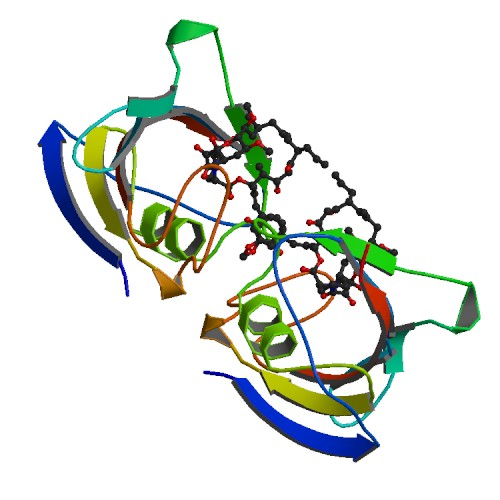
\includegraphics[width=\textwidth]{1fkj.jpg}
		\caption{1FKJ}
		\label{fig:1FKJ}
	\end{subfigure}
	~ %add desired spacing between images, e. g. ~, \quad, \qquad, \hfill etc. 
	%(or a blank line to force the subfigure onto a new line)
	\begin{subfigure}{0.4\textwidth}
		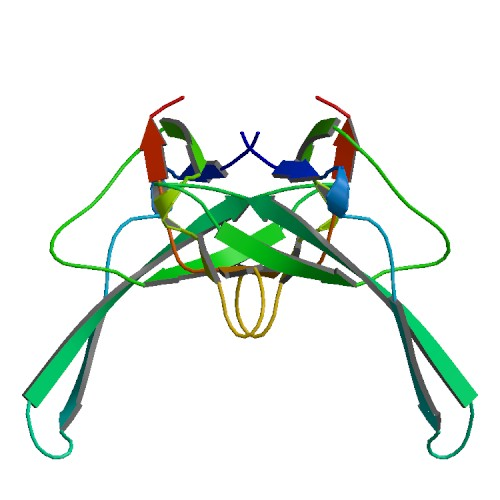
\includegraphics[width=\textwidth]{1vqb.jpg}
		\caption{1VQB}
		\label{fig:1VQB}
	\end{subfigure}
	~ %add desired spacing between images, e. g. ~, \quad, \qquad, \hfill etc. 
	%(or a blank line to force the subfigure onto a new line)
	\begin{subfigure}{0.4\textwidth}
		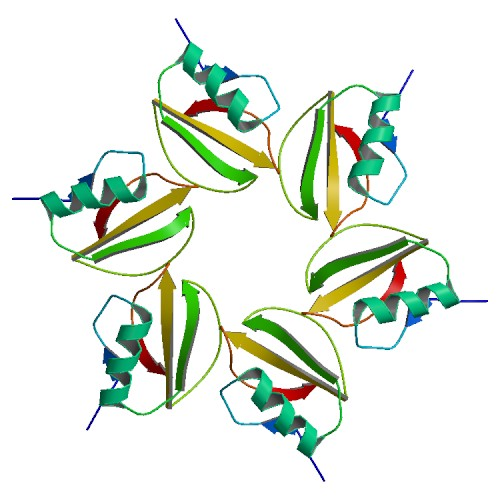
\includegraphics[width=\textwidth]{2ci2.jpg}
		\caption{2CI2}
		\label{fig:2CI2}
	\end{subfigure}
	
	\begin{subfigure}{0.4\textwidth}
		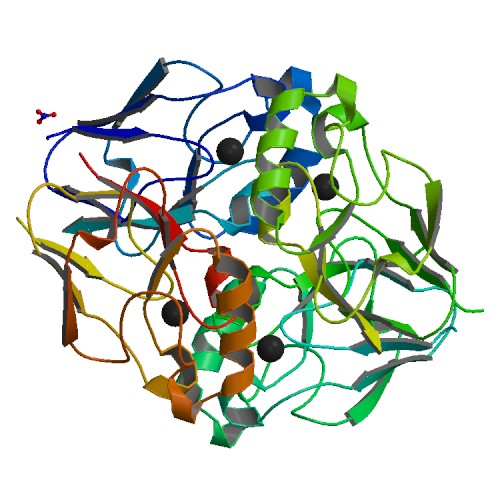
\includegraphics[width=\textwidth]{5azu.jpg}
		\caption{5AZU}
		\label{fig:5AZU}
	\end{subfigure}
	\caption{Representación de estructuras de proteínas ejemplos utilizadas para el desarrollo de meta modelos de clasificación.}
	\label{fig:proteins}
\end{figure}

Las mutaciones fueron recolectadas desde diferentes set de datos, por lo que, en caso de información ambigua, es decir, una misma mutación con diferentes respuestas, no fueron consideradas. Por otro lado, debido a que para la aplicación de la herramienta SDM se necesitaba la cadena a la cual pertenece en residuo, scripts desarrollados en Python y utilizando la librería BioPython, permitieron procesar los archivos asociados a las estructuras de las proteínas, identificadas desde el Protein Data Bank (PDB) \cite{abola1984protein}. Descartando aquellas mutaciones reportadas en las que no se encontró la cadena, obteniendo como resultante la cantidad de mutaciones reportadas para cada proteína expuestas en la Tabla \ref{cap2:tab2}.
 
\subsubsection{Evaluación del desbalance de clases y distribución de respuestas continuas}

El desbalance de clases se evaluó en aquellos set de datos con respuesta categórica, lo cual contempla, tres posibles casos: Neutral, Estable, No Estable, esto es debido a que todos los estudios donde se evalúan mutaciones, normalmente se analizan cambios que alteren la estabilidad de la proteína. En la Figura \ref{fig:desbalance}, se aprecia a modo ejemplo dos set datos y su distribución de categorías para la variable respuesta.

\begin{figure}[!h]
	\centering
	\begin{subfigure}{0.8\textwidth}
		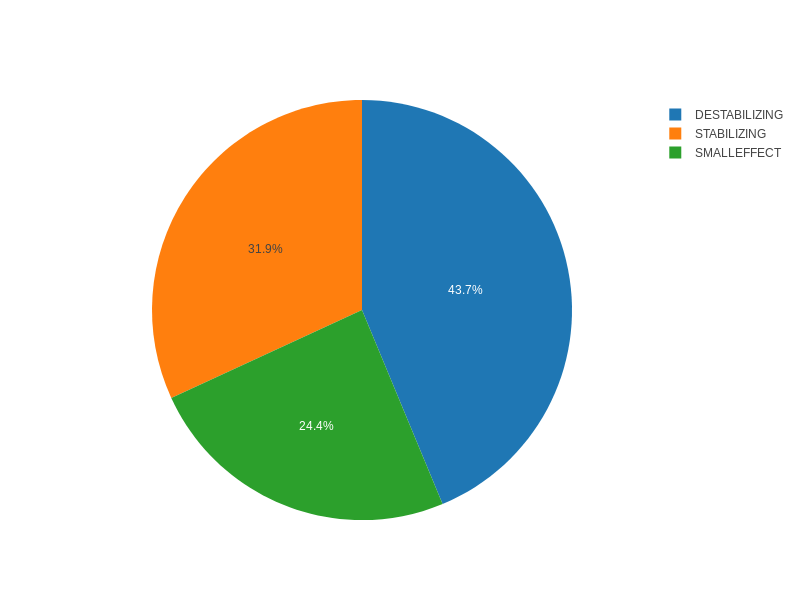
\includegraphics[width=\textwidth]{class1STN.png}
		\caption{1STN}
		\label{fig:des1}
	\end{subfigure}
	~ %add desired spacing between images, e. g. ~, \quad, \qquad, \hfill etc. 
	%(or a blank line to force the subfigure onto a new line)
	\begin{subfigure}{0.8\textwidth}
		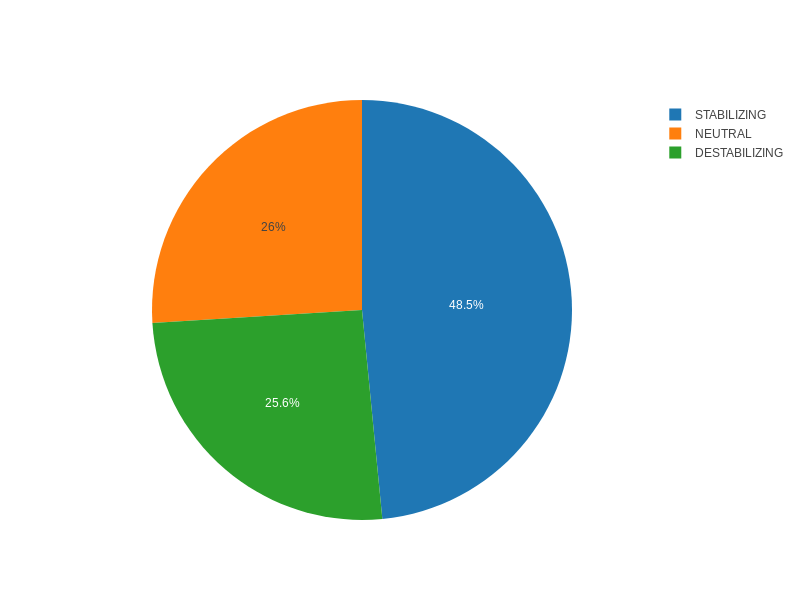
\includegraphics[width=\textwidth]{class2RN2.png}
		\caption{2RN2}
		\label{fig:des2}
	\end{subfigure}
	
	\caption{Evaluación del desbalance de clases en proteínas ejemplo.}
	\label{fig:desbalance}
\end{figure}

En las 8 proteínas en estudio para modelos de clasificación, la distribución de las categorías es similar a lo expuesta en la Figura \ref{fig:desbalance} para todas ellas, donde cerca del 50\% corresponden a mutaciones que afectan positivamente a la estabilidad, mientras que mutaciones que provocan cambios negativos o no generan diferencias, se encuentran en proporciones similares, ambas cercanas al 25\%. Si bien las proporciones son dispares, para este caso, se considera un desbalance como un elemento que representa menos de un 5\% del total de la muestra, además, dado a que la cantidad de ejemplos son elevadas, un 20\% o un 25\% implica cerca de 200 mutaciones, en promedio, que cumplen dicha característica. Además, el hecho de que exista una cantidad inferior de mutaciones no benéficas a la estabilidad viene dada a la dificultad de encontrar y reportar mutaciones que afecten negativamente a la para una proteína dado a la propensión filogenética \cite{Olivera-Nappa2011} que estos ocurran, lo cual se ve reflejado en las diferencias asociadas a cambios positivos dentro del set de mutaciones. No obstante, si bien el hecho de que la propensión filogenética indique que el cambio tiende a mejorar estabilidad, diseñar mutantes con mejoras en propiedades de interés, es un problema latente en la actualidad, de alto costo económico y computacional y con una gran demanda desde diferentes áreas del conocimiento.|

En los set de datos para el desarrollo de modelos de regresión, se evaluó la distribución de la respuesta, en este caso, valores de $\Delta\Delta\ G$ asociado a diferencias de energía libre producidas entre el residuo mutado y el original, tal que: $\Delta\ Res_{mut}\ - \Delta\ Res_{wild}\ = \Delta\Delta\ G$. 

Las distribuciones se evaluaron utilizando el test de Shapiro, con el fin de determinar si la distribución se comportaba como una normal. Para todas las proteínas estudiadas, en los 11 set de datos, las respuestas presentaron distribución normal, con valores de Shapiro sobre 0.8 y un p-value $\leq$ 0.01, lo cual indica una alta confianza estadística en los resultados presentados por dicho test.

Una visualización de las distribuciones puede generarse a partir del desarrollo de histogramas, los cuales, a modo de ejemplo se expone en la Figura \ref{fig:histogram}.

\begin{figure}[!h]
	\centering
	\begin{subfigure}{0.48\textwidth}
		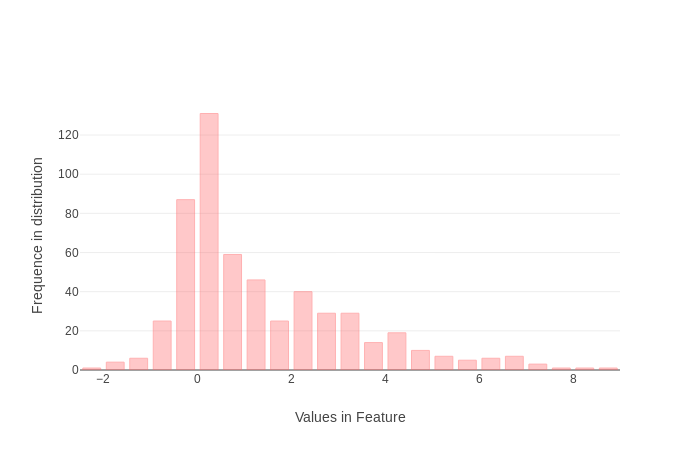
\includegraphics[width=\textwidth]{1RX4.png}
		\caption{Histograma para respuesta continua en 1RX4}
		\label{fig:hist1}
	\end{subfigure}
	~ %add desired spacing between images, e. g. ~, \quad, \qquad, \hfill etc. 
	%(or a blank line to force the subfigure onto a new line)
	\begin{subfigure}{0.48\textwidth}
		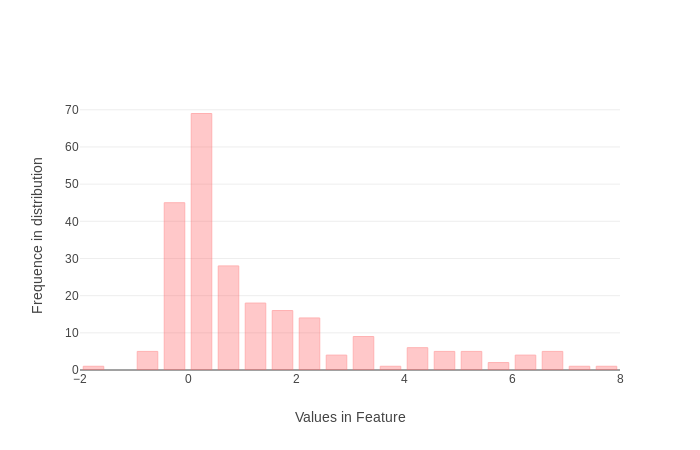
\includegraphics[width=\textwidth]{1WQ5.png}
		\caption{Histograma para respuesta continua en 1WQ5}
		\label{fig:hist2}
	\end{subfigure}
	
	\caption{Evaluación de la distribución de respuesta continua en set de datos de proteínas.}
	\label{fig:histogram}
\end{figure}

El análisis de estas características es relevante a la hora de diseñar modelos de clasificación o regresión, debido a que si existe una tendencia por una clase condiciona al clasificador a \textit{"aprender en base a la mayoría"}, por lo que puede aumentar los errores en cuanto a falsos positivos, dado a que, no se tiene la cantidad de ejemplos suficientes para una clase que permitan al modelo capturar las posibles variaciones asociadas a ésta.

Dado a los análisis de evaluación de representatividad de categorías en el set de datos y distribución de respuestas continuas, se expone que los set de datos seleccionados no presentan desbalance significativo para el caso de desarrollo de modelos de clasificación y a su vez, todas las respuestas asociadas a cambios en la energía libre para modelos de regresión, presentan distribución normal. Razón por la cual, es factible el desarrollo de modelos asociados a las respuestas presenten en los set de datos seleccionados. No obstante, sólo se ha considerado el problema del desbalance y la evaluación de distribución en la respuesta continua, una vez caracterizado los set de datos a partir de las propiedades fisicoquímicas y termodinámicas, se analizarán las características y cómo éstas condicionan la clasificación o la predicción de cambios energéticos.

\subsubsection{Caracterización del set de datos}

La caracterización del set de datos se desarrolló basándose en la descripción de una mutación a partir de sus propiedades termodinámicas y filogenéticas. Para cumplir con este objetivo, se utilizaron las herramientas SDM y MOSST.

\subsubsection{Aplicación de Meta Learning System}

El desarrollo de sistemas de meta learning para la creación de modelos se aplicó a los set de datos preparados, aplicando la metodología expuesta a lo largo de este capítulo.

Es importante mencionar, que cada set de datos se normalizó y posterior a ello, se aplicaron las etapas correspondientes a la estrategia planteada, siguiendo cada una de las etapas correspondientes: Preparación, Exploración de modelos, Selección y finalmente Creación de Meta Modelos y evaluación del desempeño. Cada uno de estos pasos se desarrollo utilizando la herramienta MLSTraining tools (\textbf{citar paper de la herramienta :D})

\subsubsection{Evaluación de los meta modelos}

Los meta modelos generados fueron evaluados con respecto a la respuesta que estos entregan, tal como se expuso previamente. Un resumen de las medidas de desempeño, tanto para los modelos de clasificación y regresión desarrollados para cada uno de los set de datos se exponen en las Tablas 

\subsubsection{Comparación de resultados obtenidos con herramientas existentes}

Es necesario generar una comparación de los resultados obtenidos con otras herramientas computacionales, con el fin de determinar si existen diferencias significativas que conlleven a mejoras en los modelos o metodologías propuestas.
 
\subsection{Herramienta computacional}

Con el fin de poder tanto los resultados de los meta modelos, los set de datos utilizados, dar a conocer la metodología planteada y disponer de una herramienta de acceso abierto, de simple uso y que permita a los usuarios entrenar sus modelos de mutantes de proteínas y compartir sus resultados con la comunidad, en caso de querer efectuarlo, se ha desarrollado una herramienta computacional web diseñada bajo la arquitectura cliente servidor en conjunto con el patrón Modelo Vista Controlador (MVC), la cual ha sido implementada bajo distintos lenguajes de programación y de etiquetado. A modo resumen del desarrollo generado, en la Tabla \ref{cap2:tab3} se exponen los componentes de software y los lenguajes bajo los cuales han sido implementados.

% Please add the following required packages to your document preamble:
% \usepackage{longtable}
% Note: It may be necessary to compile the document several times to get a multi-page table to line up properly
\begin{longtable}[c]{|l|l|l|l|}
	\hline
	\multicolumn{4}{|c|}{\textbf{Resumen de componentes en herramienta computacional}}                                                                                                                                                                                                                                                                                                                                                                                                                                                \\ \hline
	\endfirsthead
	%
	\endhead
	%
	\textbf{\#} & \textbf{Componente}                                            & \textbf{Objetivo}                                                                                                                                                                                                                                             & \textbf{Lenguaje de Programación}                                                                                                                                                  \\ \hline
	1.          & Vista                                                          & \begin{tabular}[c]{@{}l@{}}Exposición gráfica de la herramienta,\\ representa la cara visible y es quien \\ muestra los resultados y permite la \\ interacción con el usuario.\end{tabular}                                                                   & \begin{tabular}[c]{@{}l@{}}HTML5, con programación de\\ estilos utilizando frame work\\ bootstrap 3.0 y funcionalidades\\ de estilo basadas en JavaScript.\end{tabular}            \\ \hline
	2.          & \begin{tabular}[c]{@{}l@{}}Controlador \\ Cliente\end{tabular} & \begin{tabular}[c]{@{}l@{}}Es quien recibe las solicitudes o acciones\\ que efectue el usuario y las envié a servidor,\\ quien genera la respuesta y éste es quien la\\ procesa.\end{tabular}                                                                 & \begin{tabular}[c]{@{}l@{}}JavaScript, con conexión a servidor\\ por medio de Ajax y utilización del\\ plugin jQuery para los procesos de\\ carga asíncrona de datos.\end{tabular} \\ \hline
	3.          & \begin{tabular}[c]{@{}l@{}}Controlador\\ Servidor\end{tabular} & \begin{tabular}[c]{@{}l@{}}Recibe las solicitudes del controlador del\\ cliente y las procesa por medio de la inte-\\ acción con los módulos del sistema\end{tabular}                                                                                         & \begin{tabular}[c]{@{}l@{}}PhP con protocolo de respuesta\\ de transferencia de datos JSON.\end{tabular}                                                                           \\ \hline
	4.          & Modelo                                                         & \begin{tabular}[c]{@{}l@{}}Representa el conjunto de acciones que \\ procesa el servidor y están asociadas al\\ entrenamiento de modelos, consultas de \\ estados de job, solicitud de carga de resul-\\ tados, servicio de notificaciones, etc.\end{tabular} & \begin{tabular}[c]{@{}l@{}}Python en conjunto con las librerías\\ Scikit-Learn, pandas, numpy.\end{tabular}                                                                        \\ \hline
	\caption{Resumen de componentes en la herramienta computacional para el desarrollo de meta modelos y elementos bajo los cuales se encuentra implementados.}
	\label{cap2:tab3}\\
\end{longtable}

Con respecto a la visualización de la herramienta, se exponen a continuación algunos extractos de visualizaciones junto con la funcionalidad asociada.

La herramienta comienza con una interfaz inicial en la cual se encuentra la opción para cargar el set de datos y lanzar el job al sistema de colas, esto se observa en la Figura \ref{fig:h1}.

\begin{figure}[!h]
	\centering
	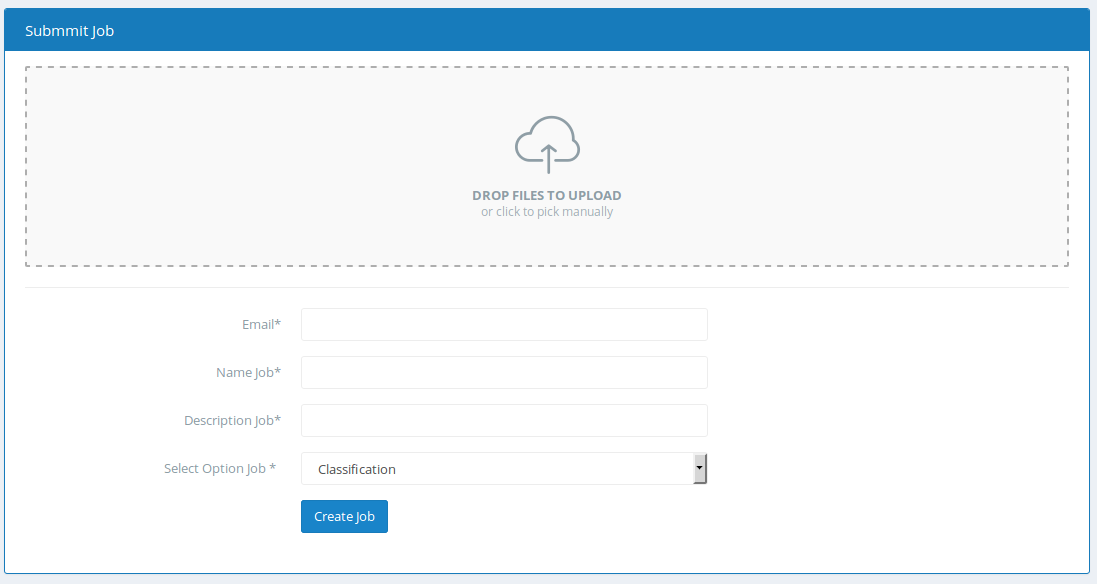
\includegraphics[scale=.4]{1.png}
		\caption{Sección de carga de archivos y generación de jobs.}
	\label{fig:h1}
\end{figure}

Por otro lado, la Figura \ref{fig:h2}, representa el módulo de búsqueda de jobs ejecutados, acción la cual, sólo debe ingresar el ID del job que se notifica por correo.

\begin{figure}[!h]
	\centering
	
\includegraphics[scale=.4]{2.png}
	\caption{Sección de búsqueda de Jobs en el sistema.}
	\label{fig:h2}
\end{figure}

En las Figuras \ref{fig:h3} y \ref{fig:h4}, se observan las visualizaciones tanto del panel de medidas de desempeño y de los modelos seleccionados por medida de desempeño, en este caso, asociadas a modelos de regresión.

\begin{figure}[!h]
	\centering
	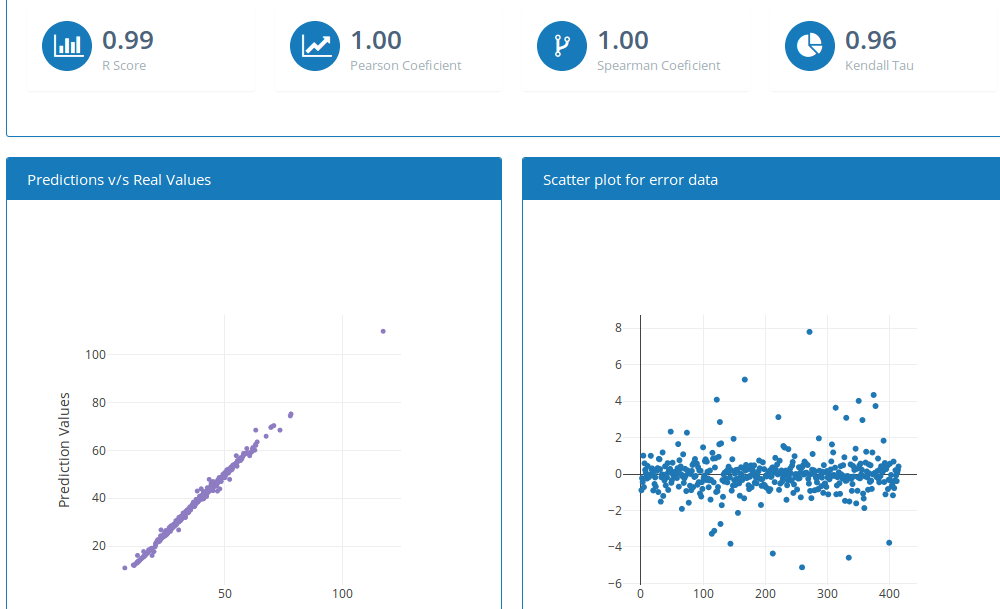
\includegraphics[scale=.4]{3.png}
	\caption{Panel asociado a las medidas de desempeño obtenidas por el modelo.}
	\label{fig:h3}
\end{figure}

\begin{figure}[!h]
	\centering
	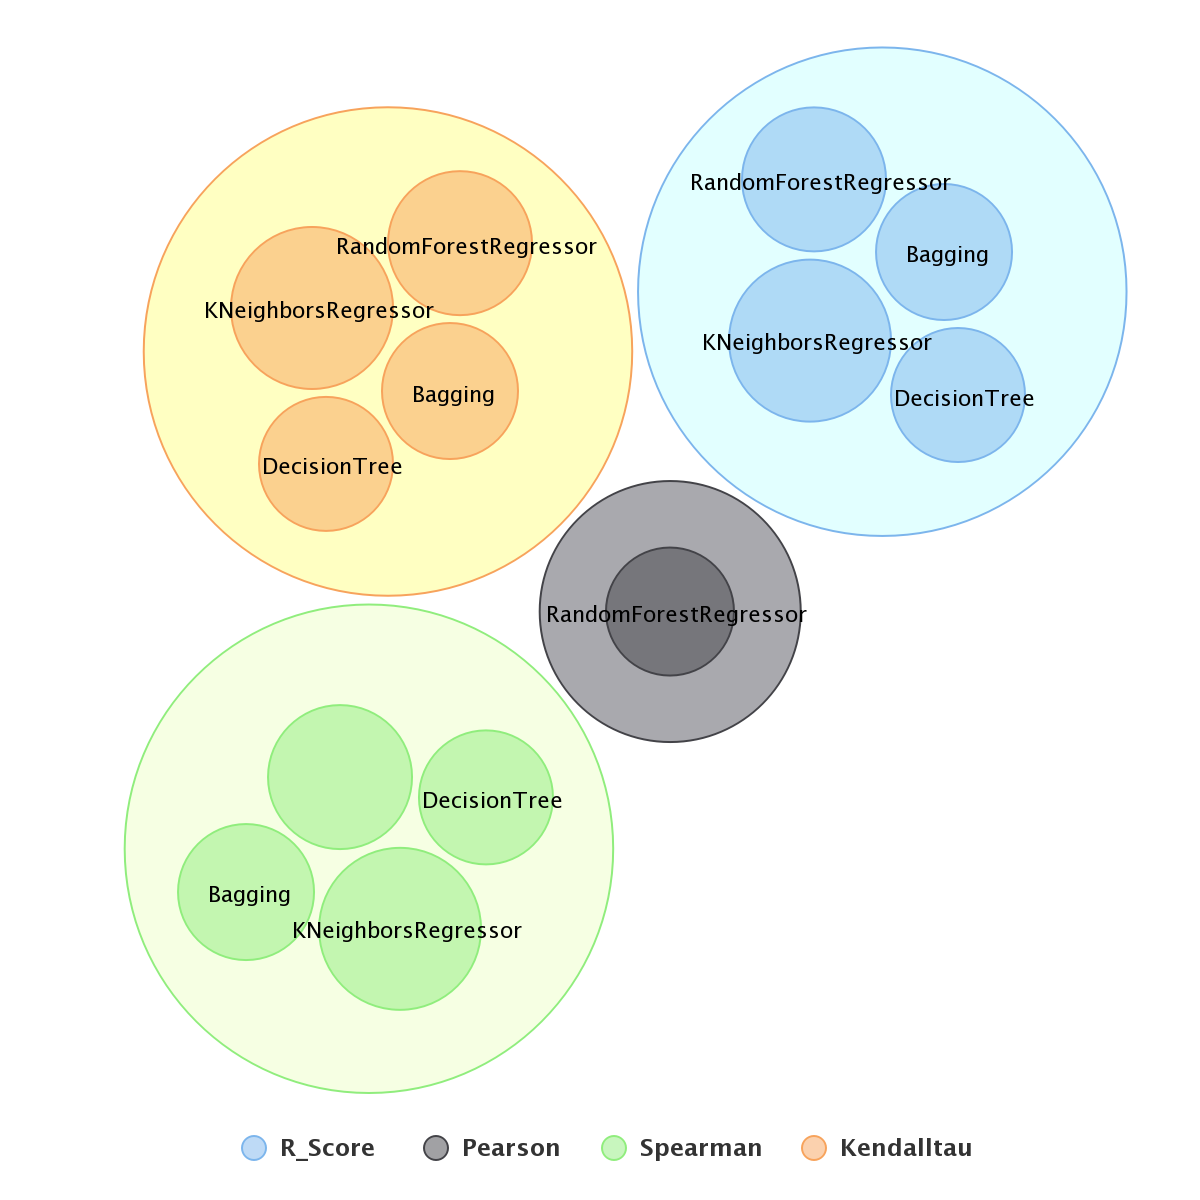
\includegraphics[scale=.3]{4.png}
	\caption{Sección de búsqueda de Jobs en el sistema.}
	\label{fig:h4}
\end{figure}

Adicional a las interfaces expuestas, la herramienta cuenta con un conjunto de secciones resúmenes, que facilitan la visualización de los resultados obtenidos, así como también las secciones correspondientes al uso de los meta modelos o la descarga de estos para ser utilizados de manera local por scripts disponibles en el repositorio del proyecto.

Finalmente se destaca, que la herramienta web se encuentra disponible con libre acceso para uso no comercial en \url{http://pesb2.cl/MLSTrainingTool/index/} con licencia GPL 3.0 y el código fuente de la librería python junto con los módulos del proyecto que componen el artefacto Modelo, se encuentra accesible desde el repositorio de la herramienta en \url{https://github.com/dMedinaO/MLSTrainingTool}.

\subsection{Caso estudio: Modelos de clasificación para evaluación de propensión clínica en mutaciones de la proteína pVHL}

Con el fin de poder evaluar la metodología planteada en un caso de estudio con diferentes respuestas y determinar una posible herramienta para uso clínico asociada a un diagnóstico preventivo y personalizado, se presenta el desarrollo de modelos de clasificación de la propensión clínica para mutantes o variantes en la proteína pVHL, responsable de la enfermedad de von Hippel Lindau.

\subsubsection{von Hippel-Lindau}

La enfermedad de von Hippel-Lindau (VHL) es un síndrome de neoplasia dominante autosómica que resulta de una mutación en la línea germinal en el gen VHL \cite{Kluijtmans1996, vogelstein2002genetic, jamaVHL, CLIFFORD200185, Maher443, KaelinJr2002, LONSER20032059}. Se caracteriza por ser un síndrome de cáncer hereditario caracterizado por el desarrollo de tumores vasculares del sistema nervioso central y retina, carcinomas renales de células claras, feocromocitomas, tumores de células de islotes pancreáticos, tumores del saco endolinfático y quistes benignos que afectan una variedad de órganos \cite{Maher443}. 

El producto canónico de la proteína VHL, \textit{pVHL} en su isoforma 1 ($pVHL_{30}$), tiene dos dominios estructuralmente diferentes, los cuales pueden ser observados en la Figura \ref{vhlView}. Un dominio desordenado de 53 aminoácidos N-terminal no necesario para la supresión tumoral y un dominio ordenado C-terminal que consiste en un dominio $\alpha$-helicoidal (residuos 155-192) y un dominio principalmente de hoja $\beta$ (residuos 63-154 y 193-204). pVHL forma un complejo ternario con las proteínas elongina C y elongina B (Complejo VCB) \cite{duan1995inhibition, Kishida4544}  el cual es crítico para la estabilidad  y la función en pVHL \cite{Schoenfeld8507}.

\begin{figure}[!h]
	\centering
	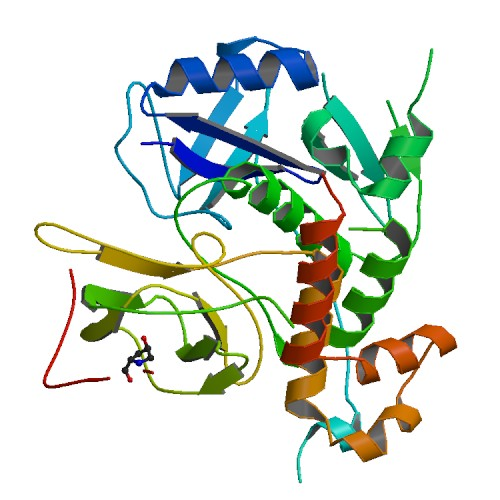
\includegraphics[scale=.5]{1lm8.jpg}
	\caption{Esquema representativo estructura VHL asociada al pdb 1LM8.}
	\label{vhlView}
\end{figure}


Las mutaciones que afectan a los residuos de unión a pVHL en elongina C se han descrito en ccRCC, lo que respalda la hipótesis de que los efectos tumorogénicos de las mutaciones de VHL se relacionan con la disfunción del complejo VCB. Por lo tanto, todo el complejo de VCB debe considerarse como una sola entidad cuando se evalúan los efectos estructurales y funcionales de las mutaciones de VHL \cite{article}.

VHL presenta una incidencia de 1 en 36.000 pacientes, los cuales se predisponen al desarrollo de hemangioblastoma retiniano, cerebeloso y espinal, quistes y carcinoma de páncreas y RCC \cite{softwareVHL}, adicional a ello, han sido documentadas, sobre 1000 mutaciones en VHL, de las cuales cerca del 52\% se desconoce su relevancia clínica o no se tiene una mayor información de ésta \cite{article}. 

Las características viscerales del trastorno incluyen quistes y carcinomas renales, los feocromocitomas, los quistes pancreáticos y los tumores neuroendocrinos, así como los cistadenomas del epidídimo y del ligamento ancho \cite{LONSER20032059}, cuyos índices de aparición se exponen en la Figura \ref{introI1}.

\begin{figure}[!h]
	\centering
	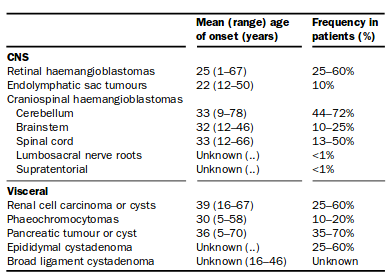
\includegraphics[scale=.8]{introVHL.png}
	\caption{Resumen de incidencias de afecciones relacionadas a VHL.}
	\label{introI1}
\end{figure}

El diagnóstico de la enfermedad de von Hippel-Lindau a menudo se basa en criterios clínicos. Los pacientes con antecedentes familiares y un hemangioblastoma del SNC (incluidos los hemangioblastomas retinianos), un feocromocitoma o un carcinoma renal de células claras son diagnosticados con la enfermedad. Los que no tienen antecedentes familiares relevantes deben tener dos o más hemangioblastomas del SNC o un hemangioblastoma del SNC y un tumor visceral (a excepción de quistes epididimarios y renales, que son frecuentes en la población general) para cumplir con los criterios diagnósticos \cite{vhlData, phillips1994neurological, LONSER20032059}.

Las correlaciones específicas de genotipo y fenotipo han surgido en las familias afectadas. Ahora se reconocen varios fenotipos familiares de la enfermedad de von Hippel-Lindau, que proporcionan información útil para examinar y aconsejar a las personas afectadas. Las familias tipo 1 tienen un riesgo muy reducido de feocromocitomas, pero pueden desarrollar todos los otros tipos de tumores generalmente asociados con la enfermedad. Las familias de tipo 2 tienen feocromocitomas, pero tienen un bajo riesgo (tipo 2A) o alto riesgo (tipo 2B) para los carcinomas de células renales. Las familias de tipo 2C solo tienen feocromocitomas, sin otros hallazgos neoplásicos de VHL \cite{LONSER20032059}.

Los avances en las pruebas genéticas para la detección de la enfermedad incluyen \textit{Southern blotting cualitativo y cuantitativo}, que se ha agregado al análisis de la secuencia de ADN. Esto mejoró para uso personal. No obstante, su reproducción es sólo con permiso de \textit{The Lancet Publishing Group}. La prueba ha aumentado la tasa de detección de mutaciones de ADN en leucocitos de sangre periférica del 75\% a casi el 100\% \cite{LONSER20032059}.

Se han desarrollado diversos software que permiten explorar el efecto de las mutaciones en las proteínas que han sido detectadas y como afectan a su estabilidad térmica y qué efectos provocan en la proteína, siendo una de éstas SDM \cite{Pandurangan2017}, el cual predice los cambios en la estabilidad esperados sobre la mutación en base a la consideración de información estructural y su secuencia, dado el uso de Tablas Específicas de entornos de sustitución (ESSTs). Por otro lado, se han desarrollado softwares que facilitan el estudio de mutaciones, mediante la evaluación de información filogenética y los cambios en la secuencia que se han observado en una familia de proteínas y una proteína de interés. Este es el caso de MOSST \cite{Olivera-Nappa2011}, el cual estima mediante cálculos matemáticos la propensión de mutaciones en la proteína a estudiar, con respecto a la familia de contraste. Otro de los software de interés que han sido desarrollados para la evaluación de mutaciones en VHL, según el riesgo de ésta es el expuesto en \cite{article}, en el cual, por medio de algoritmo Random Forest, se propone un sistema de clasificación de mutaciones según el riesgo que éstas presentan.

Dado a lo anterior, se ha denotado la falta de sistemas de clasificación de relevancia de mutaciones detectadas en VHL, las cuales han sido reportadas pero se desconoce si representarán un riesgo o no para el paciente. En base a esto y a los sistemas que se han desarrollado para trabajar con dichas mutaciones, se propone el diseño e implementación de un sistema de clasificación de mutaciones para la evaluación de la relevancia clínica de éstas ante VHL.	

\subsubsection{Set de datos y análisis de características}

El set de datos utilizado para el entrenamiento de modelos corresponde a mutaciones puntuales reportadas en la literatura \cite{softwareVHL, LONSER20032059, Maher443} de las cuales se conoce el efecto clínico, las que pueden ser clasificadas como:

\begin{enumerate}
	
	\item Relevancia  Clínica.
	\item No relevancia Clínica.
\end{enumerate}

El set de datos se compone de 256 ejemplos y la distribución de las clases es como se expone en la Figura \ref{clasesVHL}, en ella se aprecia que no existe una diferencia significativa entre las clases en cuanto a la cantidad de ejemplos, lo que implica que no existe un desbalance de clases lo cual favorece al entrenamiento de modelos de clasificación.

\begin{figure}[!h]
	\centering
	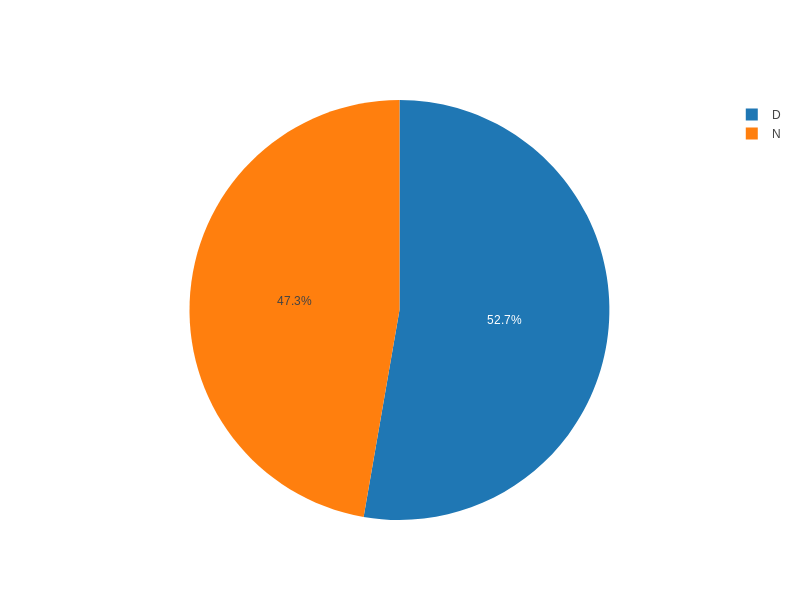
\includegraphics[scale=.4]{Clinical.png}
	\caption{Distribución de ejemplos con respecto a las clases que existen en él, D representa Relevancia clínica y N el caso contrario.}
	\label{clasesVHL}
\end{figure}

Así como se evaluó la distribución de las clases, también se hizo un análisis de las mutaciones, contemplando el residuo original y el mutado, cuya frecuencia se observa en la Figura \ref{fig:Mutaciones}. Denotando cambios asociados principalmente al aumento de prolinas y una disminución de Leucinas, el mismo fenómeno se aprecia entre los residuos de Arginina y Valina. Es posible pensar, que las variaciones entre los residuos juegan un rol fundamental en los efectos que estos provocan en la proteína dado a las características que estos presentan.  

\begin{figure}[!h]
	\centering
	\begin{subfigure}{0.48\textwidth}
		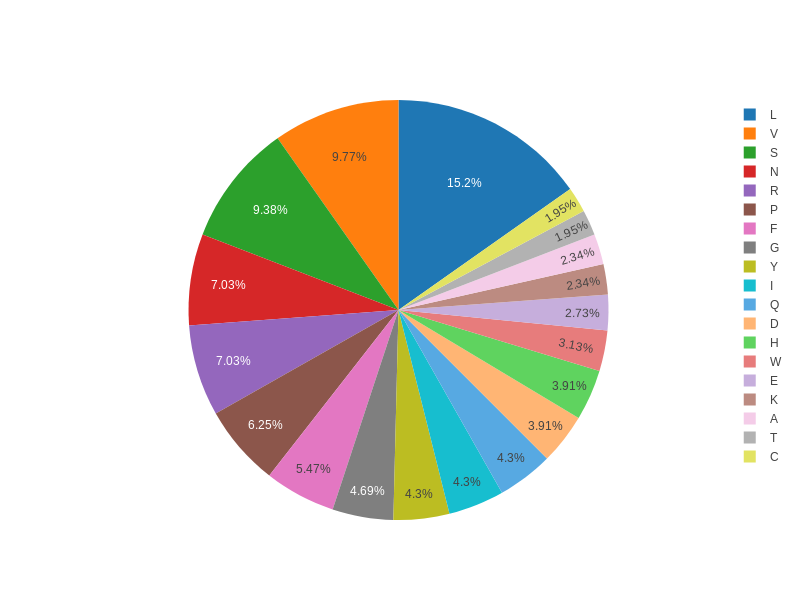
\includegraphics[width=\textwidth]{AAWt.png}
		\caption{Frecuencia de aparición de residuos wild Type en VHL.}
		\label{fig:wild}
	\end{subfigure}
	~ %add desired spacing between images, e. g. ~, \quad, \qquad, \hfill etc. 
	%(or a blank line to force the subfigure onto a new line)
	\begin{subfigure}{0.48\textwidth}
		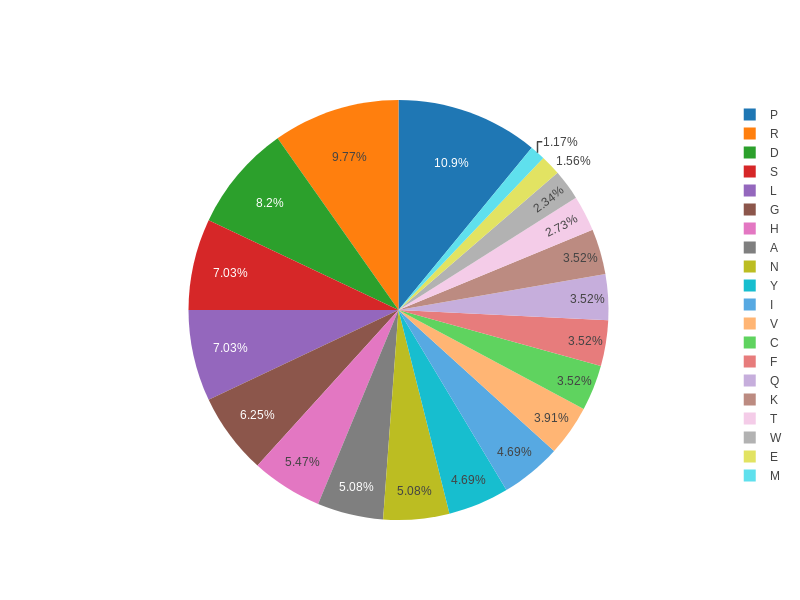
\includegraphics[width=\textwidth]{AAMt.png}
		\caption{Frecuencia de aparición de residuos mutados en VHL.}
		\label{fig:mut}
	\end{subfigure}
	
	\caption{Evaluación de la distribución de respuesta continua en set de datos de proteínas.}
	\label{fig:Mutaciones}
\end{figure}

Es importante mencionar, que análisis asociados a variaciones en las leucinas, se asocian a una leve tendencia a un cambio negativo presentando en sus casos de incidencia un total del 61\% de relevancia clínica, a su vez, al evaluar los cambios en los que aparecen prolinas, dicha tendencia aumenta a un 75\%. Denotando así, que el cambio en las propiedades fisicoquímicas de los residuos con mayor incidencia en la proteína original, provoca cambios negativos en ésta, asociándose a una clasificación negativa.

Al aplicar las herramientas MOSST y SDM al set de datos se obtuvo un conjunto de elementos descrito por 16 atributos más una respuesta, los cuales se describen en la Tabla \textbf{HACER TABLA!!!}

Dentro de los descriptores se encuentran algunos que se asocian a la mutación en si: AAWT, AAMT y posición, por otro lado, se encuentran aquellos que permiten caracterizar propiedades estructurales, termodinámicas y la evaluación del cambio de energía libre y finalmente se encuentran aquellos que permiten describir a la data a partir de sus propiedades filogenéticas, los cuales permiten generar un set de datos de clasificación con atributos de distribución continua, discreta y categórica.

Todos los atributos con distribución continua distribuyen de manera normal, según test de Shapiro, a su vez, técnicas de reducción de dimensionalidad y evaluación de características fueron aplicadas para analizar correlación de datos y relevancia de características en el set de datos por medio del aporte a la varianza o importancia a la hora de clasificar ejemplos.

Mutual information se aplicó con el fin de evaluar si existe algún tipo de correlación entre los elementos. En la Figura \ref{mutualInformation} se aprecia que existe una tendencia a no existir una relación entre las características, debido a los bajos valores de score existente entre ellos. Por otro lado, se observan correlaciones medianas (valores de mutual information cercanos a 0.5) entre los atributos asociados a la descripción de superficie accesible y los descriptores estructurales y de variación termodinámica y con un mayor énfasis en los correspondientes a las propensiones filogenéticas. Sin embargo, no existe una apreciación clara que implique remover alguna característica. 

\begin{figure}[!h]
	\centering
	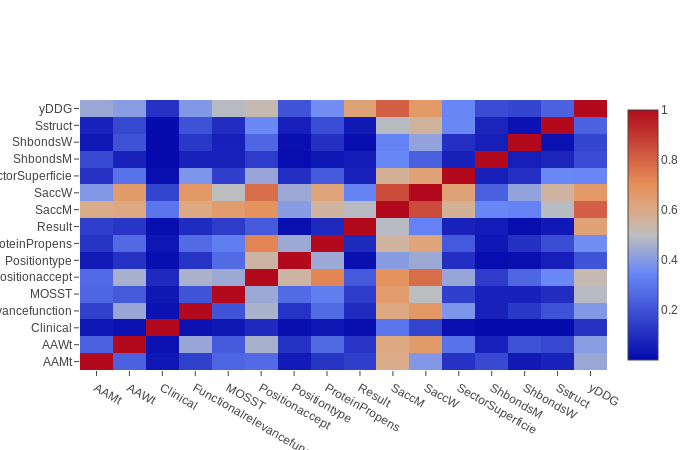
\includegraphics[scale=.6]{mutualInformation.png}
	\caption{Mutual information aplicado al set de datos para la evaluación de correlación entre los descriptores.}
	\label{mutualInformation}
\end{figure}

Análisis de componentes principales fueron aplicados para evaluar la descripción de la varianza en cuanto a las características, obteniendo que un total del 80\% de la varianza puede explicarse a partir de 8 componentes, mientras que un 90\% con un total de 12 componentes, lo cual denota que, a pesar de que son descriptores basados en diferentes propiedades y aplican diversas metodologías o estrategias para obtenerse, aportan de manera similar y no permiten explicar varianzas y clasificaciones por si mismos. Métodos basados en la evaluación de la importancia de las características a partir de indicadores basados en árboles de decisión fueron utilizados para determinar, a partir de la data, cuáles eran los atributos que más aportan a generar una clasificación. En la Figura \ref{spatial} se aprecia un ranking de importancia de características basados en análisis espacial aplicando Random Forest como algoritmo de clasificación. Los porcentajes de importancia son similares a los obtenidos mediante PCA, además se aprecia que el atributo MOSST presenta una mayor relevancia a la hora de generar una clasificación, seguidos de SaccM, yDDG y SaccW.

\begin{figure}[!h]
	\centering
	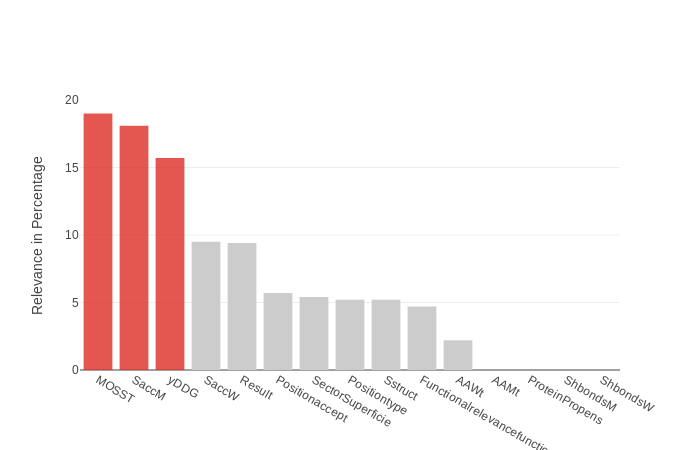
\includegraphics[scale=.5]{spatial.png}
	\caption{Análisis espacial de características empleando Random Forest como método de clasificación.}
	\label{spatial}
\end{figure}

El hecho de que dichos atributos presenten una mayor relevancia, denota que la descripción de las mutaciones basadas en propiedades termodinámicas y filogenéticas por medio de las herramientas MOSST \cite{Olivera-Nappa2011} y SDM \cite{Pandurangan2017} genera un aporte similar y permiten explicar clasificaciones, contemplando la sumatoria entre ellas un total cercano al 35\%. A su vez, las características enfocadas al porcentaje de accesibilidad a la superficie se encuentran también posicionadas dentro de los primeros puestos, denotando la relevancia de dichos sectores. Estos a su vez, presentan un rol fundamental a la hora de evaluar las interacciones entre los residuos y cómo estos participarán en la formación de alguna interacción electrostática débil permitiendo formar complejos con otras proteínas, las cuales se han visto en VHL y han sido reportadas.

Finalmente, se evaluó si los descriptores por sí solos, permiten una generar una clasificación, expresado de otra forma, si existe algún patrón inicial de combinaciones lineales que permita indicar qué atributos generarán una mejor separación de las clases en el set de datos. Para ello, visualizaciones al set de datos empleando coordenadas paralelas y SPLOM fueron desarrolladas. 

Coordenadas paralelas permite seguir una traza a la visualización de los atributos y determinar rangos donde se prefiere o tiende a alguna clasificación para los ejemplos. En la Figura \ref{parallel} se aprecia dicho análisis y se expone que no existe una tendencia clara a una clasificación o rangos de valores para clases particulares. Esto denota que si bien existe una alta variabilidad de la información, no hay rasgos o patrones característicos que faciliten el desarrollo de clasificadores.

\begin{figure}[!h]
	
	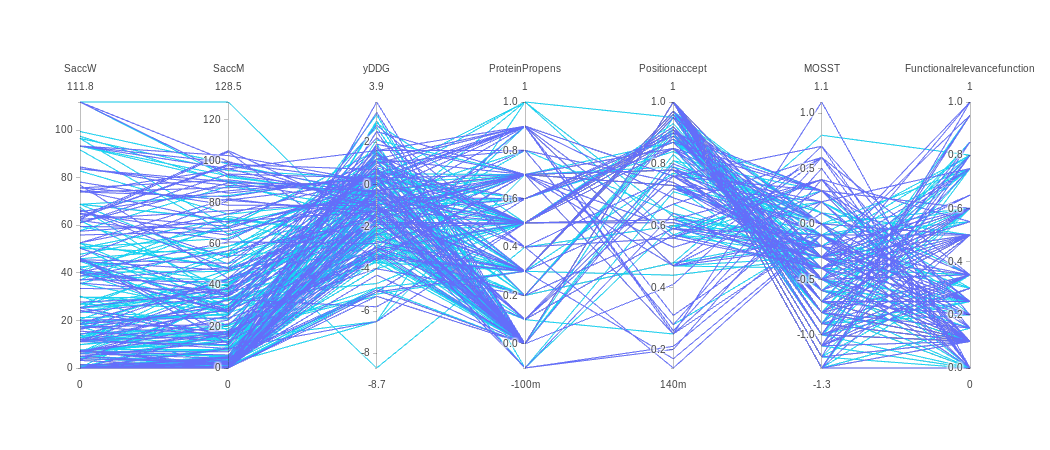
\includegraphics[scale=.45]{parallel.png}
	\caption{Análisis de características mediante visualización de coordenadas paralelas.}
	\label{parallel}
\end{figure}

Las matrices SPLOM (Scatter plot matrix) permite plotear las variables entre sí con el fin de evaluar si existe alguna separación entre algún posible descriptor. En la Figura \ref{scatter} se aprecia la matriz de ploteo para las características con distribución continuas presentes en el set de datos, denotando lo expuesto mediante coordenadas paralelas.

\begin{figure}[!h]
	
	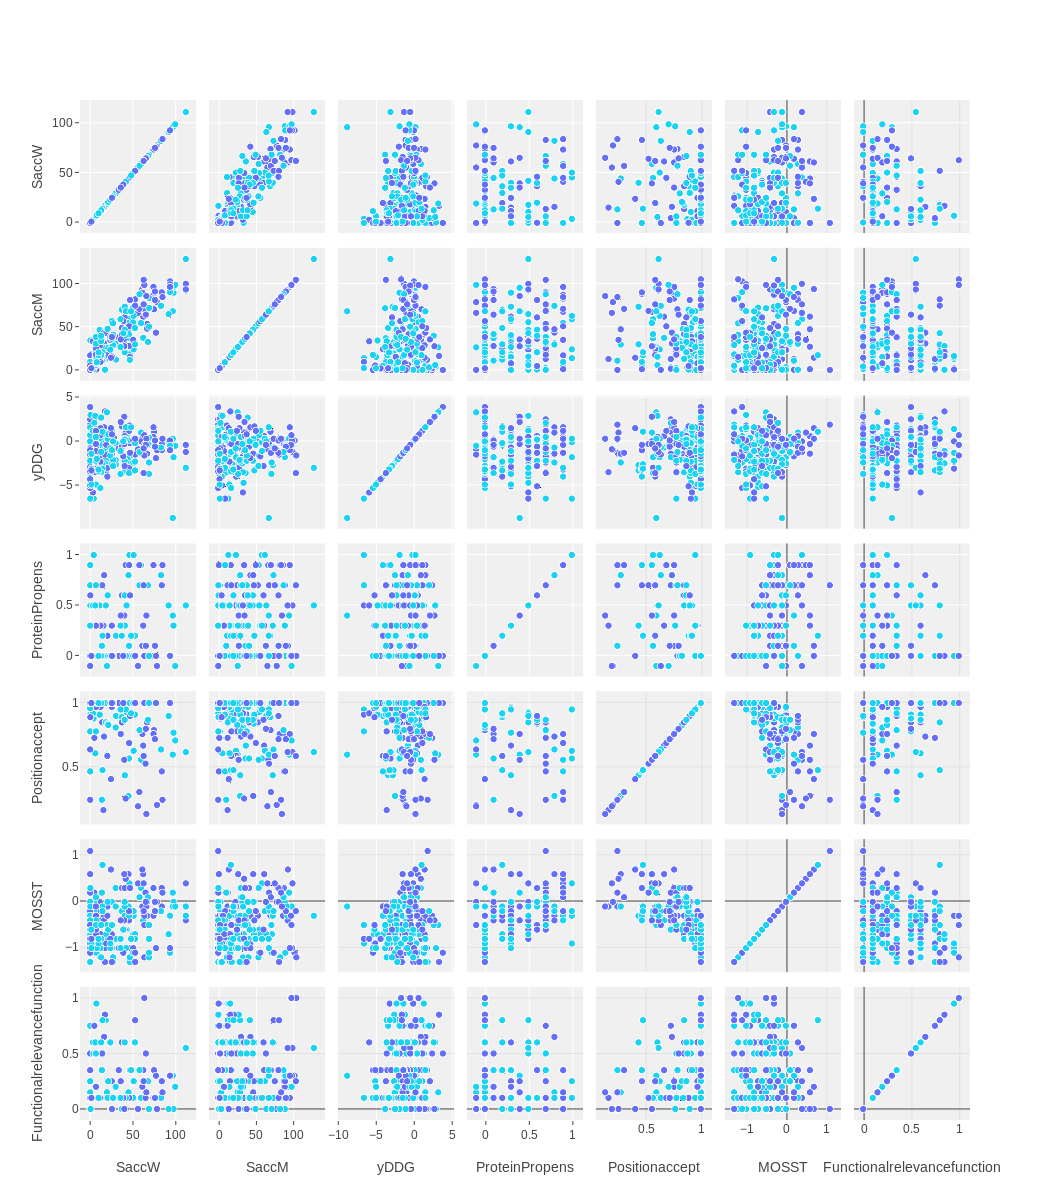
\includegraphics[scale=.45]{splom.png}
	\caption{Análisis de características mediante visualización a través de matrices de ploteo.}
	\label{scatter}
\end{figure}

En ambos casos, se observa que no existen patrones visuales que permitan generar una separación entre las clases existentes. Si se entrenan modelos de clasificación a partir de algoritmos de aprendizaje supervisado, es muy probable que estos tiendan a ser azarosos y sus desempeños sean pobres, debido a que no existen tendencias claras de separación y estrategias como aplicar hiperplanos, evaluar en base a distancia, seleccionar probabilidades y el uso de las características como indicadores de separación no brindarán buenos resultados.

\subsubsection{Entrenamiento de modelos}

El set de datos se sometió a la metodología expuesta durante este capítulo, generando una fase de preparación de los datos en base a la codificación por Ordinal Encoder de las variables categóricas. La normalización de los datos implicó el uso de escala normal dado a que las distribuciones de las características presentaban comportamiento de ese estilo. 

2886 modelos fueron evaluados durante la fase de exploración, obteniendo distribuciones de medidas de desempeño con comportamiento normal, las cuales, a modo de ejemplo, se expone en la Figura \ref{accuracyBad} la distribución de la Exactitud (Accuracy). 

\begin{figure}[!h]
	\centering
	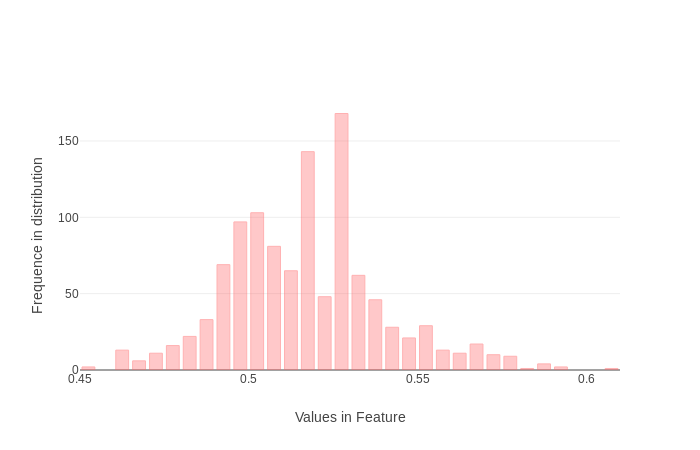
\includegraphics[scale=.6]{dist.png}
	\caption{Distribución de valores de Exactitud obtenidos en la fase exploratoria de la metodología implementada.}
	\label{accuracyBad}
\end{figure}

Los valores obtenidos para la exactitud presentan un margen entre 0.45 y un máximo cercano a 0.6, estos indican claramente que los diferentes modelos desarrollados son azarosos y no serán de confianza a la hora de evaluar nuevos ejemplos. Adicional a la exactitud, los valores de las restantes medidas de desempeño no presentan un panorama muy alentador o con indicios de mejoras para el modelo.

Un resumen general de estas métricas se aprecia en la Tabla \ref{tab:summaryStatistic}, en la cual se observa claramente que los valores máximos son muy bajos con respecto a lo que se espera de un sistema de clasificación con utilidad diagnóstico médico.

% Please add the following required packages to your document preamble:
% \usepackage{longtable}
% Note: It may be necessary to compile the document several times to get a multi-page table to line up properly
\begin{longtable}[c]{|l|l|l|l|l|l|}
	\hline
	\multicolumn{6}{|c|}{\textbf{Estadísticos resumen para medidas de desempeño en modelos de clasificación}}                                                                                                                                                                                                                                                                                   \\ \hline
	\endfirsthead
	%
	\endhead
	%
	\multicolumn{1}{|c|}{\textbf{Feature}} & \multicolumn{1}{c|}{\textbf{Average}} & \multicolumn{1}{c|}{\textbf{\begin{tabular}[c]{@{}c@{}}Standar\\ Deviation\end{tabular}}} & \multicolumn{1}{c|}{\textbf{Variance}} & \multicolumn{1}{c|}{\textbf{\begin{tabular}[c]{@{}c@{}}Max\\ Value\end{tabular}}} & \multicolumn{1}{c|}{\textbf{\begin{tabular}[c]{@{}c@{}}Min\\ Value\end{tabular}}} \\ \hline
	\textbf{Accuracy}                      & 0.51                                  & 0.02                                                                                      & 0.0005                                 & 0.60                                                                              & 0.45                                                                              \\ \hline
	\textbf{f1}                            & 0.40                                  & 2.62                                                                                      & 6.9039                                 & 0.65                                                                              & 0.0                                                                               \\ \hline
	\textbf{Precision}                     & 0.32                                  & 0.17                                                                                      & 0.0317                                 & 0.65                                                                              & 0.0                                                                               \\ \hline
	\textbf{Recall}                        & 0.29                                  & 0.19                                                                                      & 0.0369                                 & 0.9                                                                               & 0.0                                                                               \\ \hline
	\caption{Tabla resumen estadísticos obtenidos en la fase exploratoria de modelos de clasificación para el set de datos VHL.}
	\label{tab:summaryStatistic}\\
\end{longtable}

Los resultados obtenidos eran de esperarse debido a la poca separación o disgregación existente entre los datos o a la falta de presentar una claridad o diferenciación entre los atributos con el fin de \textit{"facilitar el aprendizaje"} a los modelos de clasificación. También se evaluó la transformación de variables a componentes mediante técnicas de PCA, con el fin de maximizar la variabilidad de los datos y generar características con propiedades ortogonales entre ellas. Sin embargo, dicha transformación implicó resultados similares a los obtenidos inicialmente. 

Las siguientes fases de la metodología permitieron aumentar las medidas de desempeño, en un 10\% aproximadamente, obteniendo meta clasificadores con performance cercanas al 70\%, lo cual, sigue siendo modelos no utilizables en el diagnóstico clínico. 

Con el fin de mejorar las medidas de desempeño y teniendo conocimiento sobre la estructura de la proteína y los sitios de interacción que ésta posee, se decide utilizar dicha información con el motivo de generar sub conjuntos de datos enfocados en sitios específicos o sectores de interacción particulares, es decir, enfocando el desarrollo de modelos de clasificación a diferentes mutantes reportadas para distintas superficies de pVHL, siguiendo una estrategia similar a \cite{Capriotti2005}, en el cual subdividen los set de datos con respecto al tipo de estructura secundaria en el cual se encuentra.

De manera similar, se trabajó con el set de datos y se subdividió en base a sus sectores de interacción, a modo de esquematizar la ubicación de las superficies, en la Figura \ref{surface} cuáles son dichas entidades, las cuales permitieron generar set de datos superficie-específicos.

\begin{figure}[!h]
	\centering
	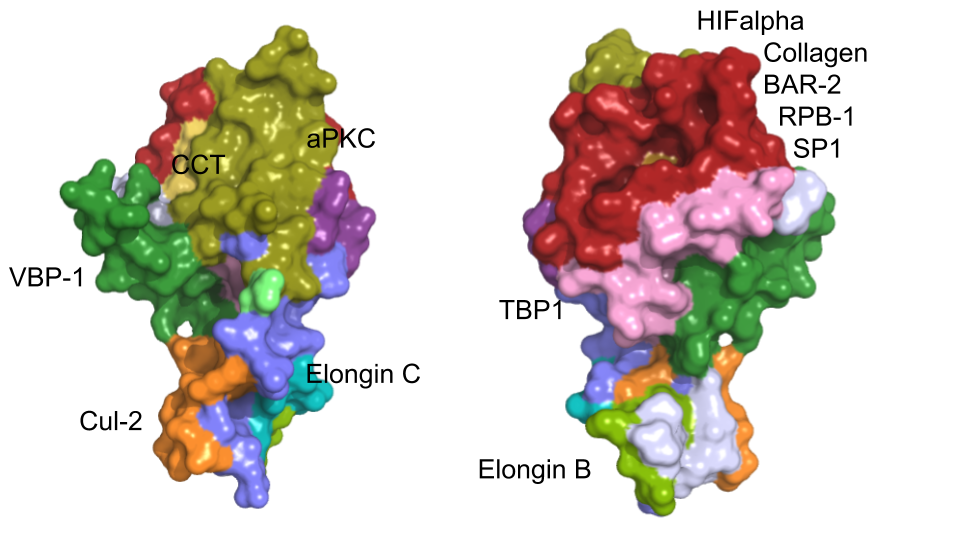
\includegraphics[scale=.4]{surface.png}
	\caption{Superficies de interacción reportadas para pVHL y utilizadas como criterio de formación de set de datos superficie-específicos.}
	\label{surface}
\end{figure}

En la Figura \ref{surface} se aprecian 12 superficies de interacción, adicional a ellas, se agrega una división de no interacción o de sitios en donde no han sido reportadas interacciones. Una distribución de los ejemplos y el tamaño de set de datos para dichas divisiones se expone en la Figura 

\begin{figure}[!h]
	\centering
	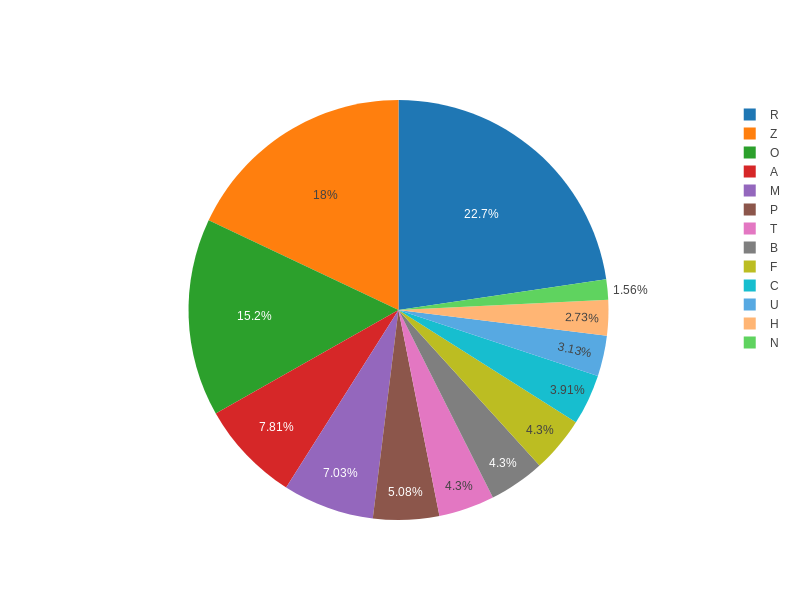
\includegraphics[scale=.5]{SectorSuperficie.png}
	\caption{Distribución de cantidad de ejemplos por set de datos para división generada en base a superficie de interacción.}
	\label{surfac2}
\end{figure}

En base a dicho planteamiento, se aplica la metodología diseñada a cada set de datos empleando diferentes tipos de validación con respecto a la cantidad de ejemplos existentes en cada set de datos. Así, si el número de elementos en la división fuese menor a 20, se emplea Leave one Out como método de validación, mientras que si es mayor a 20 pero menor a 50 se emplea Validación cruzada con un \textit{K=5} y finalmente, para los casos restantes, se utiliza un valor de \textit{K=10}.

\subsubsection{Meta modelos obtenidos en base set de datos superficie-específicos}

13 Meta modelos fueron desarrollados en base a las particiones generadas según la superficie de interacción y aplicando la metodología dispuesta previamente.

En la Tabla \ref{tab:metaModels} se expone un resumen de la cantidad de componentes por cada meta modelo, las ponderaciones obtenidas y las medidas de desempeños globales para el conjunto de datos de entrenamiento de VHL.

% Please add the following required packages to your document preamble:
% \usepackage{longtable}
% Note: It may be necessary to compile the document several times to get a multi-page table to line up properly
\begin{longtable}[c]{|l|l|l|l|l|l|}
	\hline
	\multicolumn{6}{|c|}{\textbf{Resumen de Meta modelos obtenidos para divisiones por superficie de interacción}}                                                                                                                                                                                 \\ \hline
	\endfirsthead
	%
	\endhead
	%
	\multicolumn{1}{|c|}{\textbf{Sector}} & \multicolumn{1}{c|}{\textbf{Ejemplos}} & \multicolumn{1}{c|}{\textbf{\begin{tabular}[c]{@{}c@{}}Nro\\ Modelos\end{tabular}}} & \multicolumn{1}{c|}{\textbf{Accuracy}} & \multicolumn{1}{c|}{\textbf{Recall}} & \multicolumn{1}{c|}{\textbf{Precision}} \\ \hline
	A                                     & 20                                     & 7                                                                                   & 0,82                                   & 1                                    & 0,786                                   \\ \hline
	B                                     & 11                                     & 8                                                                                   & 0,81                                   & 1                                    & 0,78                                    \\ \hline
	C                                     & 10                                     & 5                                                                                   & 0,83                                   & 1                                    & 0,79                                    \\ \hline
	F                                     & 11                                     & 4                                                                                   & 0,83                                   & 0,94                                 & 0,82                                    \\ \hline
	H                                     & 7                                      & 5                                                                                   & 0,82                                   & 1                                    & 0,78                                    \\ \hline
	M                                     & 18                                     & 9                                                                                   & 0,81                                   & 1                                    & 0,81                                    \\ \hline
	N                                     & 4                                      & 5                                                                                   & 1                                      & 1                                    & 1                                       \\ \hline
	O                                     & 39                                     & 4                                                                                   & 0,75                                   & 0,88                                 & 0,77                                    \\ \hline
	P                                     & 13                                     & 12                                                                                  & 0,74                                   & 0,87                                 & 0,8                                     \\ \hline
	R                                     & 58                                     & 3                                                                                   & 0,85                                   & 1                                    & 0,8                                     \\ \hline
	T                                     & 11                                     & 5                                                                                   & 0,82                                   & 1                                    & 0,8                                     \\ \hline
	U                                     & 8                                      & 5                                                                                   & 1                                      & 1                                    & 1                                       \\ \hline
	Z                                     & 46                                     & 4                                                                                   & 0,74                                   & 1                                    & 0,83                                    \\ \hline
	\textbf{Totales}                      & \textbf{256}                           & \textbf{76}                                                                         & \textbf{0,83}                          & \textbf{0,976}                       & \textbf{0,83}                           \\ \hline
	\caption{Meta modelos obtenidos para cada superficie de interacción aplicando la metodología de Meta Learning System.}
	\label{tab:metaModels}\\
\end{longtable}

Las medidas globales para el sistema se obtuvieron en base a la ponderación de las medidas de desempeño individuales de cada subdivisión generada versus el aporte de ejemplos que ésta posee. Así se obtiene un modelo general para clasificaciones de mutaciones en VHL con una Precisión y Exacitud de un 83\% y un Recall de 1. Denotando así, que el hecho de generar divisiones implica una mejora considerable en cuanto a las medidas de desempeño obtenidas al utilizar todo el conjunto de elementos.

Cada sector de superficie presenta diferentes métricas, número de ejemplos y cantidad de modelos. A su vez, incluso se diferencian en los algoritmos que componen el sistema de clasificación, siendo en algunos casos una tendencia al uso de Random Forest mientras que en otros Support Vector Machine e inclusive KNN. 

Los algoritmos que componen los meta modelos permiten explicar el porqué se genera la clasificación, debido a los fundamentos en los cuales se desarrollan estos. En el caso de KNN se expone la cercanía de un nuevo ejemplo a otro ya clasificado, SVM traza hiperplanos para generar la clasificación mientras que Random Forest genera árboles de decisión basados en las características con el fin de obtener el resultado. Esto facilita la explicación de la asociación de clases a nuevos ejemplos y genera un sistema claro a la hora de entender los resultados obtenidos.

A modo de ejemplo y con el fin de ilustrar los resultados obtenidos, en la Figura X se ilustra un esquema representativo de los algoritmos que componen el meta modelo y la matriz de confusión de éste.

Si bien, el inducir divisiones en el set de datos presentó mejoras considerables en cuanto a las medidas de desempeño, provoca la interrogante de si éstas mejoraron sólo por disminuir la cantidad de ejemplos en el set de datos o porque la división en base a superficies de interacción es un real aporte a la generación de modelos de clasificación en VHL.

Diversas estrategias de división del set de datos fueron aplicadas a la hora de validar la división en base a superficies de interacción. Al aplicar algoritmos de aprendizaje no supervisado se obtuvieron particiones que fueron sometidas a la metodología planteada en este algoritmo. Sin embargo, todos los resultados obtenidos se basan en modelos de redes neuronales, por lo que, a pesar de que los resultados obtenidos eran levemente inferiores a los expuestos en la Tabla \ref{tab:metaModels} no fueron consideradas debido a que no entregaban una justificación en cuanto a la clasificación de nuevos ejemplos dado el hecho de actuar en torno a cajas negras.

Por otro lado, algoritmos recursivos para generar particiones fueron implementados, seleccionando las divisiones en base a métricas de clustering. No obstante, los resultados no superan a los obtenidos por la división basada en superficies de interacción. Finalmente, divisiones aleatorias manteniendo el número de grupos y a variando la cantidad de ejemplos fueron generado. No obstante, aquellos meta modelos que presentaron resultados similares a los obtenidos se basaban en algoritmos de redes neuronales, no facilitando la explicación de nuevas clasificaciones \footnote{Para más detalles de esto, revisar el artículo X en donde se exponen el desarrollo de modelos de clasificación para VHL.} \textbf{Debo citar al paper de VHL-Hunter acá}.


\section{Conclusiones finales}



